%TODO: CORREGIR COMANDOS PARA QUE SE VEAN CON VERB
%TODO: INTENTAR QUITAR LA MORRAYA QUE NO SIRVA
%TODO: INTENTAR NO REPETIR TANTAS COSAS EN EL EJERCICIO 3
%TODO: REVISAR DOCUMENTO PARA FALLOS ORTOGRAFICOS/GRAMATICALES
\documentclass{article}
\usepackage[utf8]{inputenc}
\usepackage[spanish]{babel}
\usepackage{graphicx, graphics, float, hyperref}
\usepackage{listings}
\usepackage[a4paper, total={6in, 10in}]{geometry}

\title{SSO Práctica 1}
\author{Andrés Merlo Trujillo}
\date{}
\hypersetup{
    colorlinks=true,
    linkcolor=black,
}

\begin{document}

\maketitle

\tableofcontents

\newpage
\addcontentsline{toc}{section}{Ejercicio 1}
\section*{Ejercicio 1}
A continuación, voy a explicar el formato y el significado de cada uno de los campos. Para ello, voy a dividir cada archivo en subsecciones:

\addcontentsline{toc}{subsection}{/etc/passwd}
\subsection*{/etc/passwd}
\textbf{Formato:} \verb|nombre_login:contra_encriptada:UID:GID:comentario:shell|

\begin{figure}[H]
    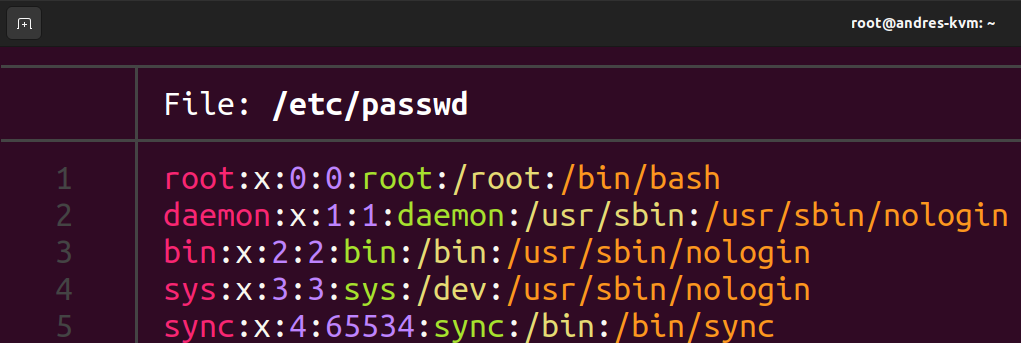
\includegraphics[width=\textwidth]{imagenes/passwdfile.png}
    \caption{Ejemplo de entradas en el archivo.}
\end{figure}

\bigskip

Este fichero está formado por líneas de 7 campos separados por ``:''. Los campos y sus significados son los siguientes:

\begin{enumerate}
    \item \textbf{Nombre de login: }Nombre de usuario.
    \item \textbf{Contraseña encriptada opcional: }Contraseña encriptada del usuario.
    Si este campo tiene la letra ``x'' minúscula, significa que la contraseña se almacena en ``/etc/shadow''.

    Si se encuentra vacío, significa que no hace falta contraseña para autenticar.

    Si comienza en exclamación, significa que la contraseña ha sido bloqueada.

    Además, si contiene una exclamación o un asterisco, significa que el usuario no podrá usar la contraseña para iniciar sesión (pero puede usar otro medio).

    \item \textbf{User ID numérico: }ID del usuario.
    \item \textbf{Group ID numérico: }ID del grupo al que pertenece.
    \item \textbf{Nombre de usuario o campo de comentario: }Este campo sirve para poder poner un comentario sobre el usuario (por ejemplo: acción que realiza, para evitar confusión con dos usuarios similares, etc.).
    \item \textbf{Directorio home del usuario: }Directorio que será el home privado del usuario. Además sirve para poner la variable de entorno ``\$HOME''
    \item \textbf{Interprete opcional de comando de usuario: }Shell que usará el usuario por defecto (bash, sh, zsh, fish, etc.). Además, pondrá la variable de entorno ``\$SHELL'' a este valor.
\end{enumerate}

\addcontentsline{toc}{subsection}{/etc/group}
\subsection*{/etc/group}
\textbf{Formato: }\verb|nombre_grupo:contra:GID:usuario1,usuario2,...|

\begin{figure}[H]
    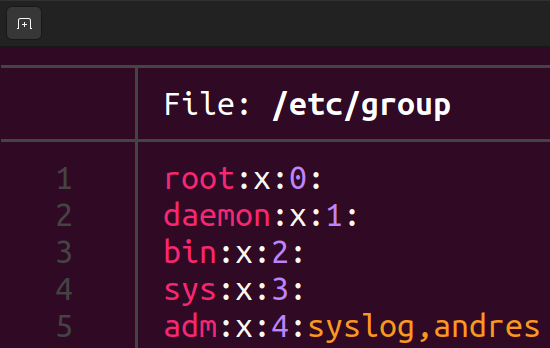
\includegraphics[width=\textwidth]{imagenes/groupfile.png}
    \caption{Ejemplo de entradas en el archivo.}    
\end{figure}

\bigskip

Este fichero está formado por 4 campos separados por ``:''. EL significado de cada campo es el siguiente:

\begin{enumerate}
    \item \textbf{Nombre del grupo: }Nombre del grupo. Este nombre debe ser único en el sistema.
    
    %REVISAR ESTE CAMPO
    \item \textbf{Contraseña: }Contraseña del grupo. Si es una letra ``x'' minúscula significa que la contraseña encriptada se encuentra en ``/etc/gpasswd''.
    \item \textbf{Group ID: }Indica el ID del grupo. Este valor debe ser único en el sistema.
    \item \textbf{Usuarios: }Lista de usuarios separados por coma (``,'') los cuales son miembros del grupo. 
\end{enumerate}

\addcontentsline{toc}{subsection}{/etc/shadow}
\subsection*{/etc/shadow}
\textbf{Formato: }\verb|login:pass:last_change:min_age:max_age:pass_warn:pass_inact:acc_exp:reserved|

\begin{figure}[H]
    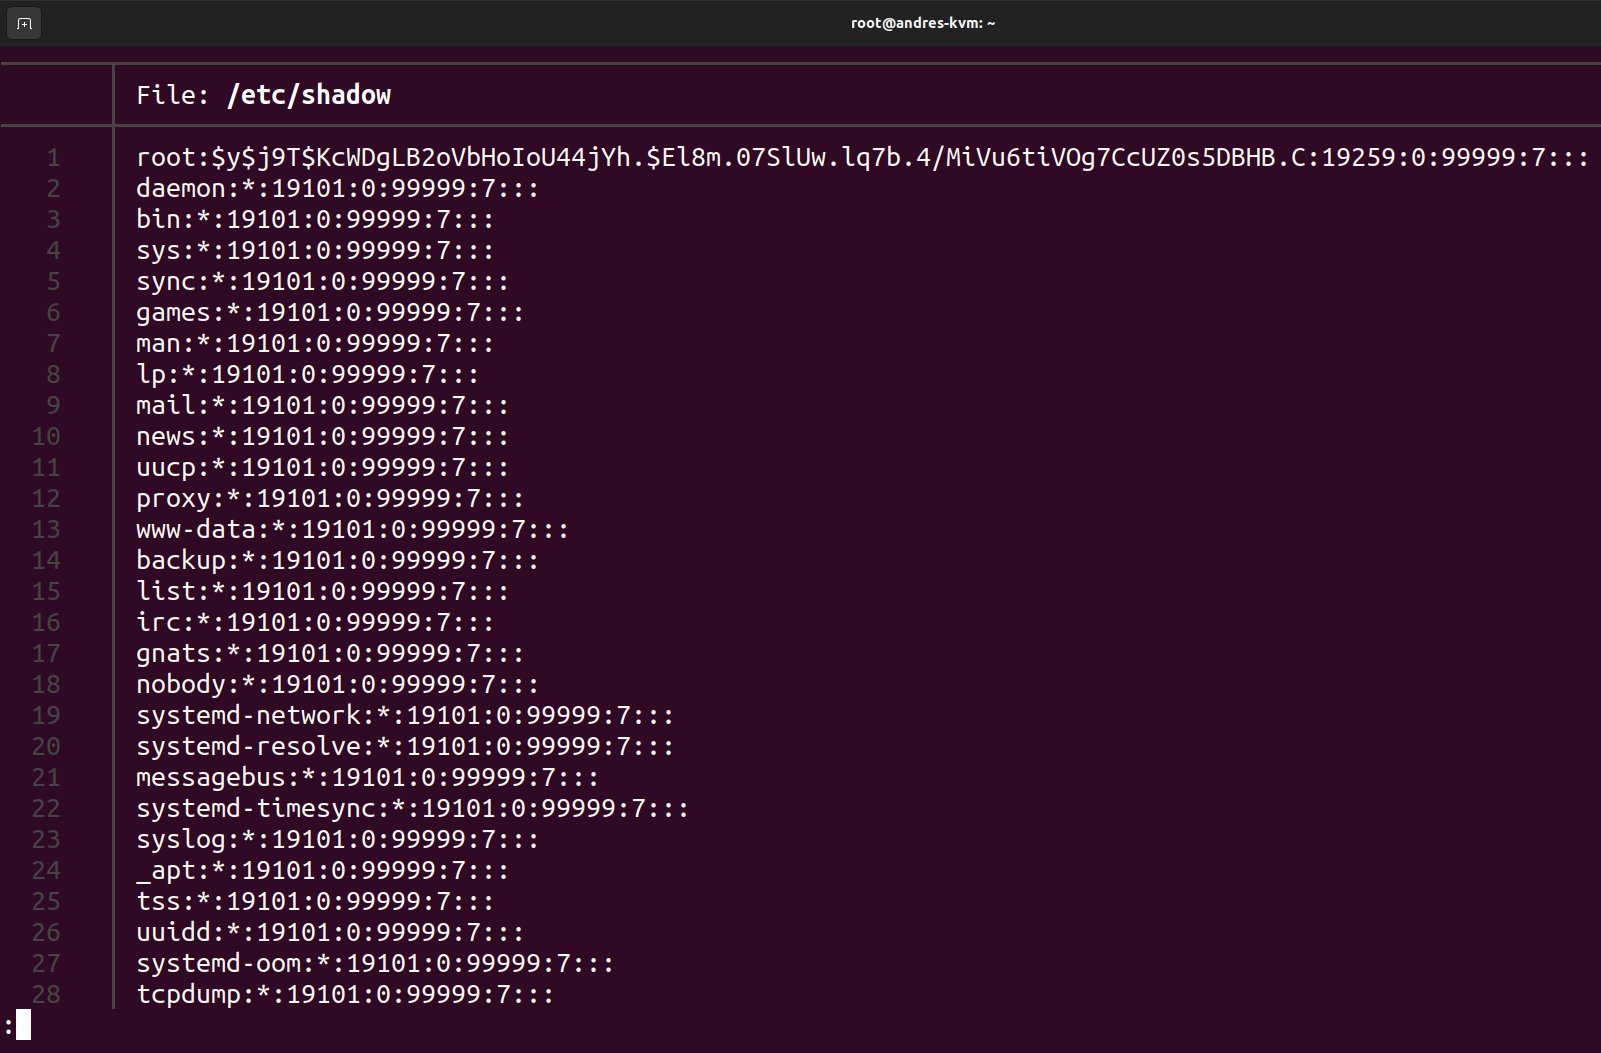
\includegraphics[width=\textwidth]{imagenes/shadowfile.png}
    \caption{Ejemplo de entradas en el archivo.}    
\end{figure}

\bigskip

Este fichero está formado por líneas de 9 campos separados por ``:''. Los campos y sus significados son los siguientes:

\begin{enumerate}
    \item \textbf{login name (nombre de login): }Nombre de la cuenta del usuario. Debe existir en el sistema.
    
    %Hablar de la encriptacion concreta que tiene (quizas sea un salteo)
    \item \textbf{encrypted password (contraseña encriptada): }Contraseña encriptada del usuario especificado en ``login name''. Si este campo está vacío, significa que ese usuario no requiere contraseña para iniciar sesión. 
    
    Además, en caso de que la contraseña comience con una exclamación (``!''), significa que la contraseña ha sido bloqueada.

    Por último, si la contraseña contiene el carácter de exclamación mencionado anteriormente o asterisco (``*''), significa que no puede iniciar sesión (si es exclamación también se cumple lo de arriba).

    \item \textbf{date of last password change (fecha del último cambio de contraseña): }El último cambio de contraseña, expresado como el número de días desde el epoch (1 de enero de 1970).
    
    Además, si el valor es 0 significa que el usuario debe cambiar la contraseña en el próximo login.

    %comprobar este parrafo
    En cambio, si el campo está vacío significa que las contraseñas no tienen edad (y por tanto no se cumplen estas restricciones).

    \item \textbf{minimum password age (edad mínima de la contraseña): }Número de días que el usuario tiene que esperar antes de poder cambiar la contraseña de nuevo. Un valor 0 ó vacío indica que no hay un mínimo de días.
    \item \textbf{maximum password age (edad máxima de la contraseña): }Número máximo de días en los cuales la contraseña ``caduca'' (tiene que cambiarla). Al pasar este número de días, el sistema pedirá al usuario que cambie la contraseña.
    
    Si el valor máximo es mayor que el del campo anterior, el usuario no podrá cambiar su contraseña.

    Por último, si el campo está vacío, se deshabilitara este servicio junto con ``password warning period'' y ``password inactivity period''.

    \item \textbf{password warning period (periodo de advertencia de la contraseña): }El número de días antes de que la contraseña ``caduque'' durante los cuales se le  advierte al usuario.
    
    Un valor 0 o cadena vacía indica que no habrá advertencias.

    \item \textbf{password inactivity period (periodo de inactividad de la contraseña): }Número de días después de que la contraseña haya ``caducado'' en el cual debería ser aceptada. Al pasar este periodo, el usuario no podrá iniciar sesión.
    
    Un campo vacío indica que no se cumple esta regla.

    \item  \textbf{account expiration date (fecha de expiración de la cuenta): }La fecha en la que la cuenta expira. Esta fecha se expresa como el número de días desde el epoch.
    
    La diferencia con la expiración de una contraseña es que, si la cuenta expira, no podrá iniciar sesión de ninguna forma, mientras que si la contraseña expira, tendrá otros medios para iniciar sesión.

    El campo vacío indica que la cuenta no expira. Además, no se debe usar el valor 0, ya que se puede interpretar como que la cuenta expira en el epoch o que no expira.

    \item \textbf{reserved field (campo reservado): }Este campo está reservado para usos futuros.
\end{enumerate}


\addcontentsline{toc}{subsection}{/etc/gshadow}
\subsection*{/etc/gshadow}
\textbf{Formato: }\verb|group_name:encrypted_pass:admin1,admin2,...:member1,member2,...|

\bigskip

\begin{figure}[H]
    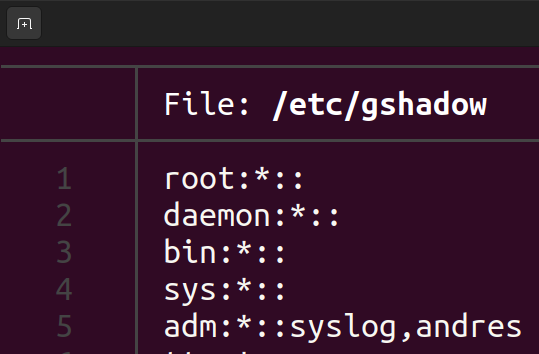
\includegraphics[width=\textwidth]{imagenes/gshadowfile.png}
    \caption{Ejemplo de entradas en el archivo.}    
\end{figure}

Este fichero está también formado por 4 campos separados por el símbolo ``:''. El significado de cada campo es el siguiente:

\begin{enumerate}
    \item \textbf{Nombre del grupo: }Nombre del grupo. Debe existir en el sistema.
    \item \textbf{Contraseña encriptada: }Contraseña encriptada que sirve para que un usuario que no es miembro del grupo obtenga los permisos.
    
    Si el campo está vacío, entonces cualquier usuario puede obtener los privilegios del grupo.

    Si la contraseña comienza por una exclamación, significa que esta está bloqueada.

    Si contiene una exclamación o asterisco, los usuarios no podrán acceder al grupo si no están en él.

    \item \textbf{Administradores: }Lista de usuarios separados por coma que puede realizar operaciones como cambiar la contraseña del grupo o administrar los usuarios del mismo.
    \item \textbf{Miembros: }Lista de usuarios separados por coma. Los miembros del grupo pueden acceder al mismo sin necesitar la contraseña.
\end{enumerate}

\addcontentsline{toc}{section}{Ejercicio 2}
\section*{Ejercicio 2}
En este ejercicio se pide modificar el valor de la variable ``LOGIN\_TIMEOUT'' y comprobar sus efectos con un usuario nuevo que se haya creado manualmente.

Para ello, modifico la variable, que estaba por defecto a 60 segundos:

\begin{figure}[H]
    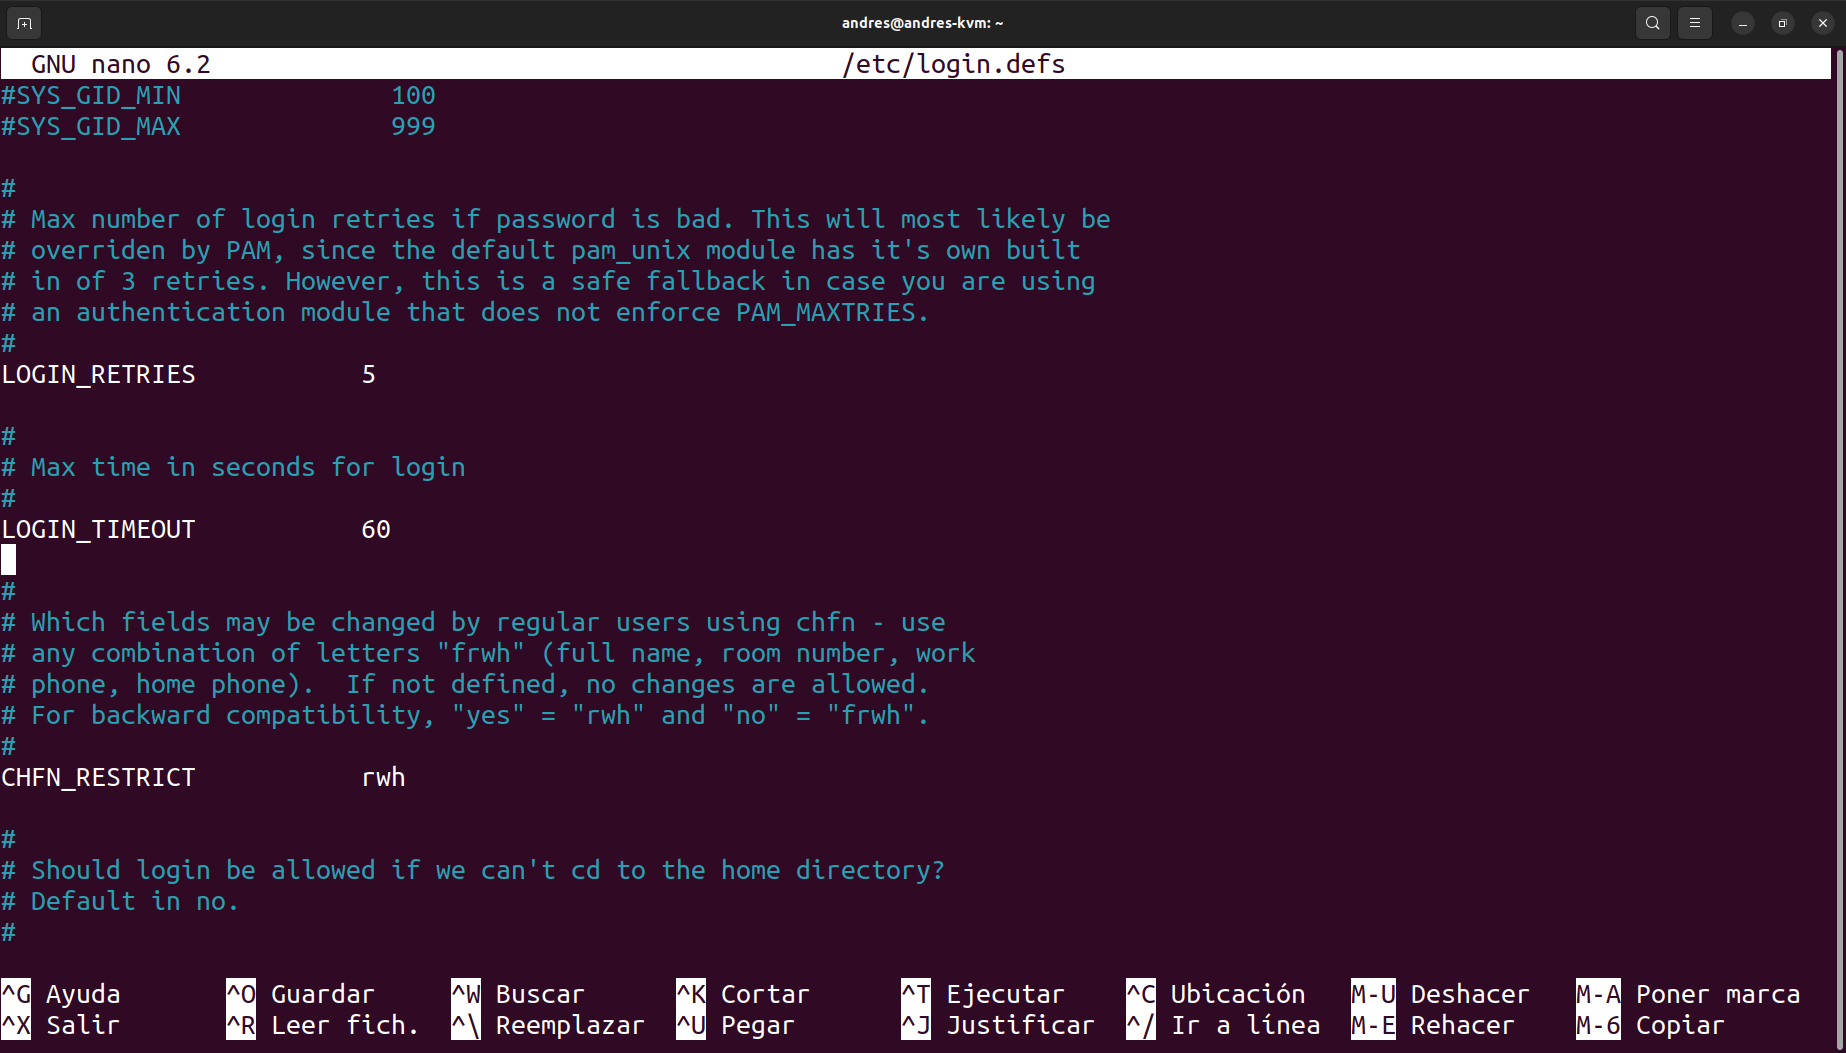
\includegraphics[width=\textwidth]{imagenes/tout60.png}
    \caption{Valor por defecto.}
\end{figure}

Y lo cambio a otro valor, por ejemplo, 5 segundos:

\begin{figure}[H]
    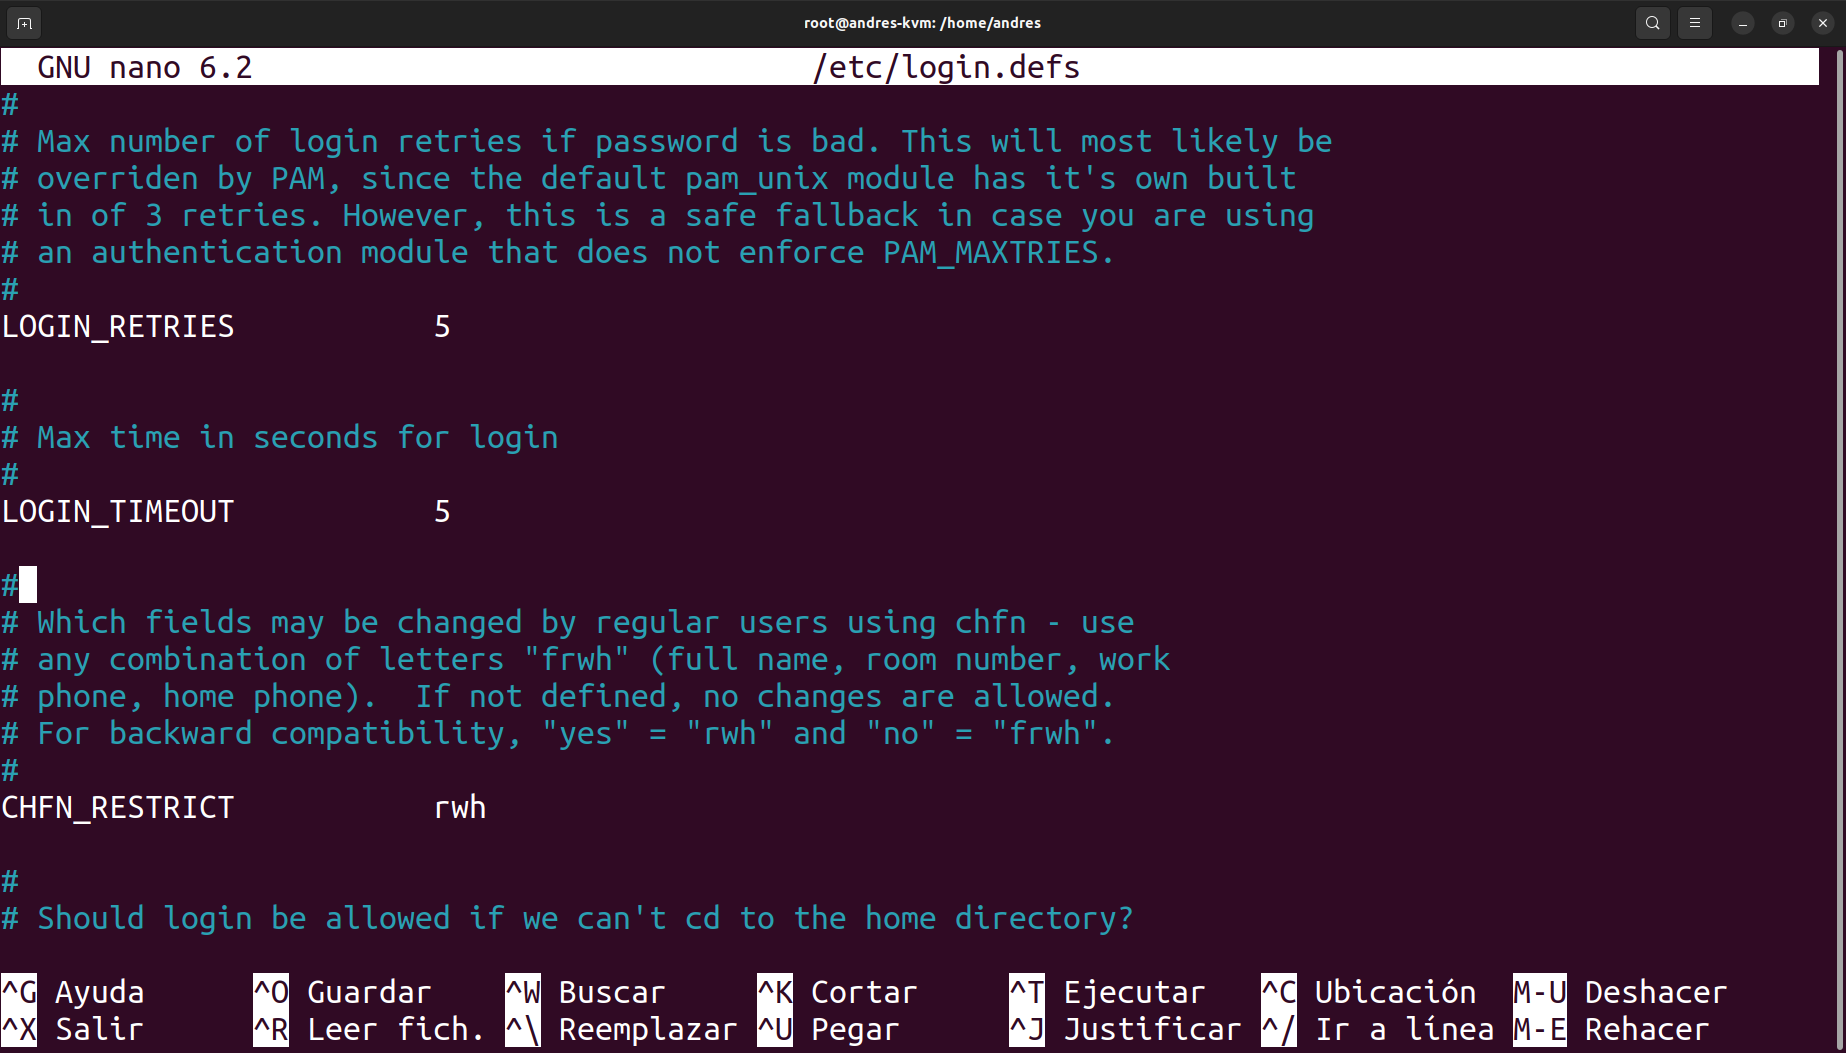
\includegraphics[width=\textwidth]{imagenes/tout5.png}
    \caption{Valor cambiado a 5 segundos.}
\end{figure}

A continuación, creo el usuario llamado ``prueba'', le cambio la contraseña y hago login con él desde la terminal. Cuando se encuentre en la parte de pedir la contraseña de este usuario nuevo, se espera un tiempo hasta que la terminal devuelva un mensaje:

\begin{figure}[H]
    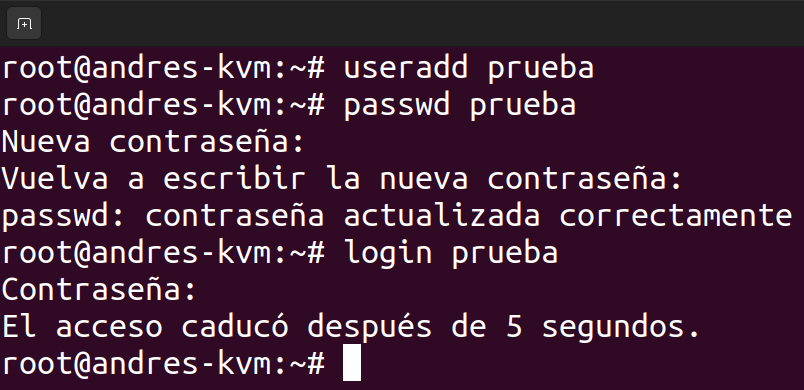
\includegraphics[width=\textwidth]{imagenes/tout5login.png}
\end{figure}

Como se puede ver, pone que han pasado 5 segundos y el acceso ha caducado.

Ahora, pruebo con otro valor, por ejemplo \textbf{12} segundos:

\begin{figure}[H]
    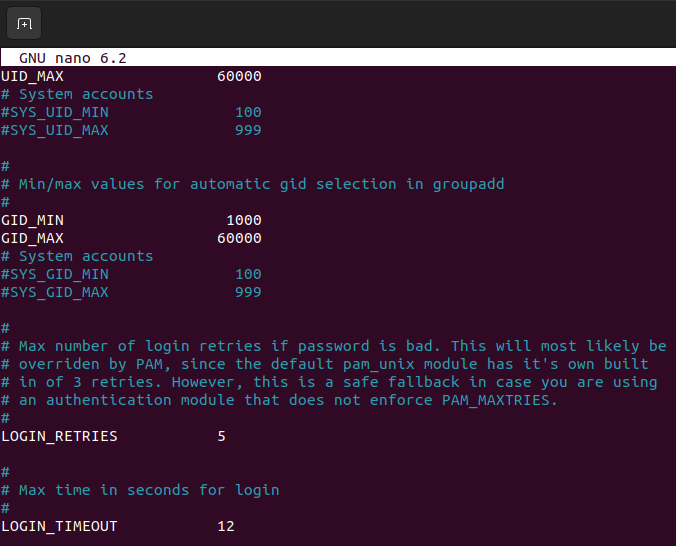
\includegraphics[width=\textwidth]{imagenes/tout12.png}
\end{figure}

E intento iniciar sesión de nuevo con el usuario ``prueba'' y espero en la parte de la contraseña.

\begin{figure}[H]
    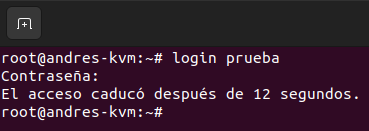
\includegraphics[width=\textwidth]{imagenes/tout12login.png}
\end{figure}

Como se puede ver, el timeout ahora es distinto.


\addcontentsline{toc}{section}{Ejercicio 3}
\section*{Ejercicio 3}
En este ejercicio se pide crear un archivo y darle, mediante un ACL, permisos de lectura y escritura al usuario creado (en mi caso sigue siendo ``prueba'').

Para ello, mediante la orden ``touch'' creo el archivo denominado ``ejercicio3''.

Ahora bien, al menos en Ubuntu 22.04 no están las órdenes ``getacl/setacl'', sino que se llaman ``getfacl/setfacl''. El resultado no varía y tienen las mismas sintaxis.

\begin{figure}[H]
    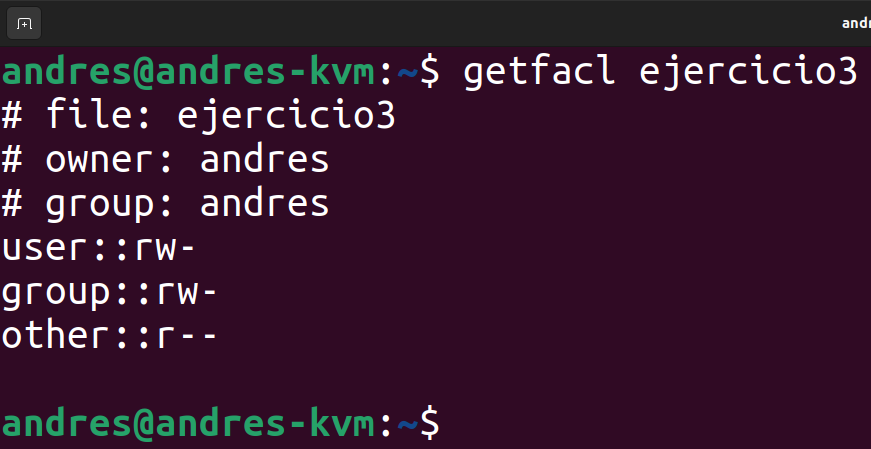
\includegraphics[width=\textwidth]{imagenes/getfaclorg.png}
    \caption{Se puede ver que solo el usuario ``andres'' tiene los permisos}
\end{figure}


Ahora, con la orden \verb|setfacl -m u:prueba:rw ejercicio3| se le dará al usuario ``prueba'' permisos ``rw''. Y de nuevo mostramos con ``getfacl'' el archivo anterior:

\begin{figure}[H]
    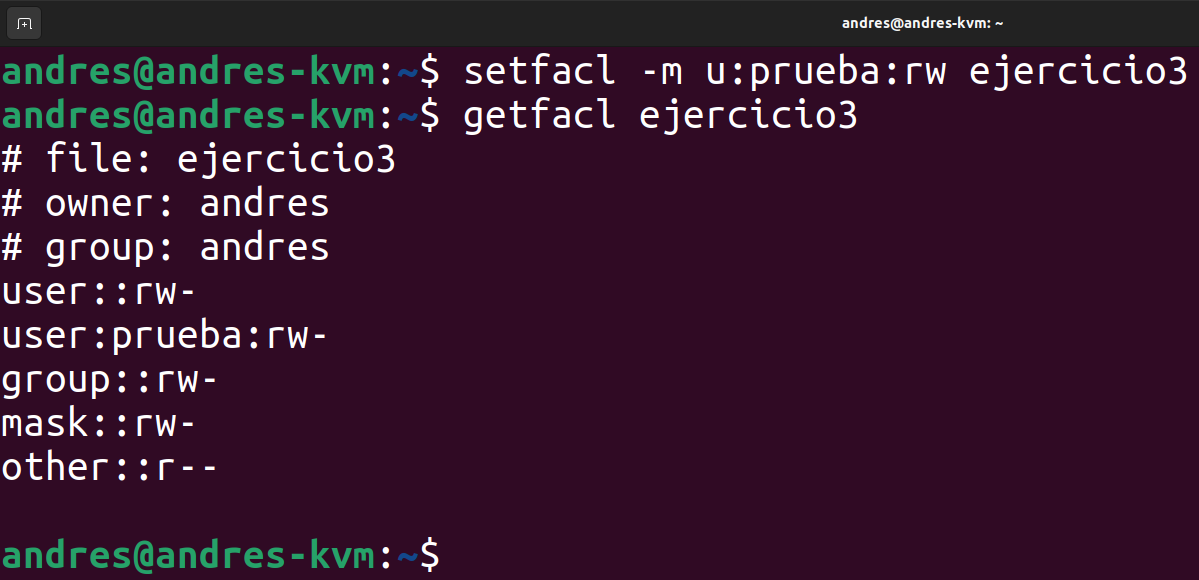
\includegraphics[width=\textwidth]{imagenes/getfaclnew.png}
    \caption{se puede ver que solo el usuario ``andres'' tiene los permisos}
\end{figure}

Como se puede observar, ahora aparece una línea que indica que el usuario ``prueba'' tiene permisos ``rw''.


\addcontentsline{toc}{section}{Ejercicio 4}
\section*{Ejercicio 4}
Con el comando ``ls'' muestro los archivos que se encuentran en el directorio ``/etc/pam.d'':

\begin{figure}[H]
    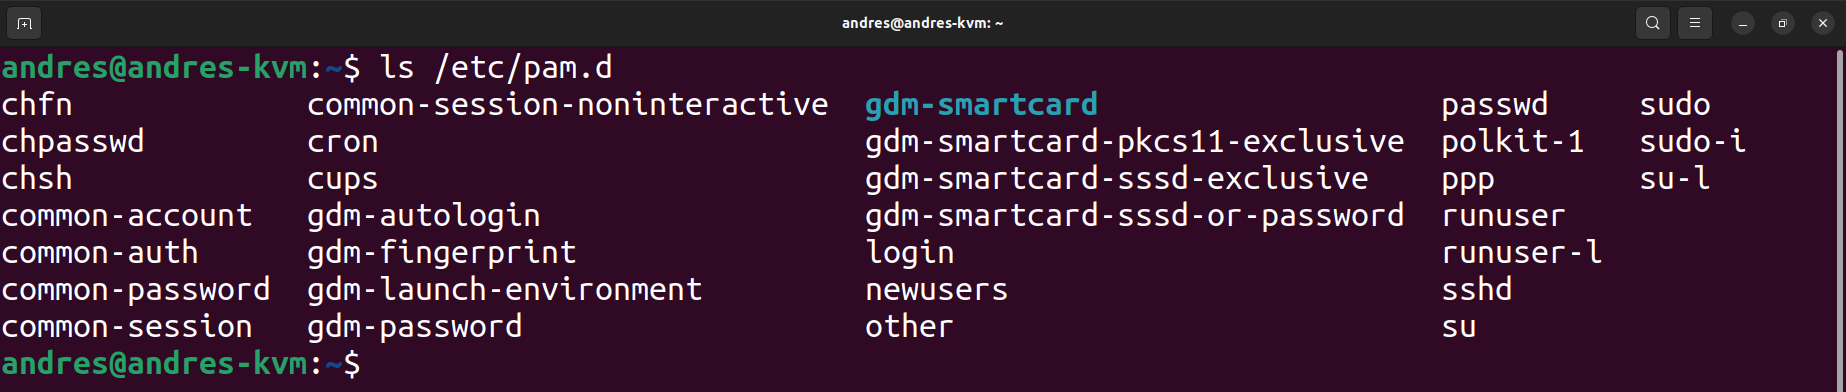
\includegraphics[width=\textwidth]{imagenes/lspam.png}
\end{figure}

A continuación explicaré dos archivos:

\addcontentsline{toc}{subsection}{/etc/pam.d/chfn}
\subsection*{/etc/pam.d/chfn}
Permite cambiar la información personal de un usuario tales como: el nombre, el número de teléfono, de habitación, etc. Estos datos luego pueden ser leídos por comandos como ``finger''.

El contenido del archivo es:

\begin{figure}[H]
    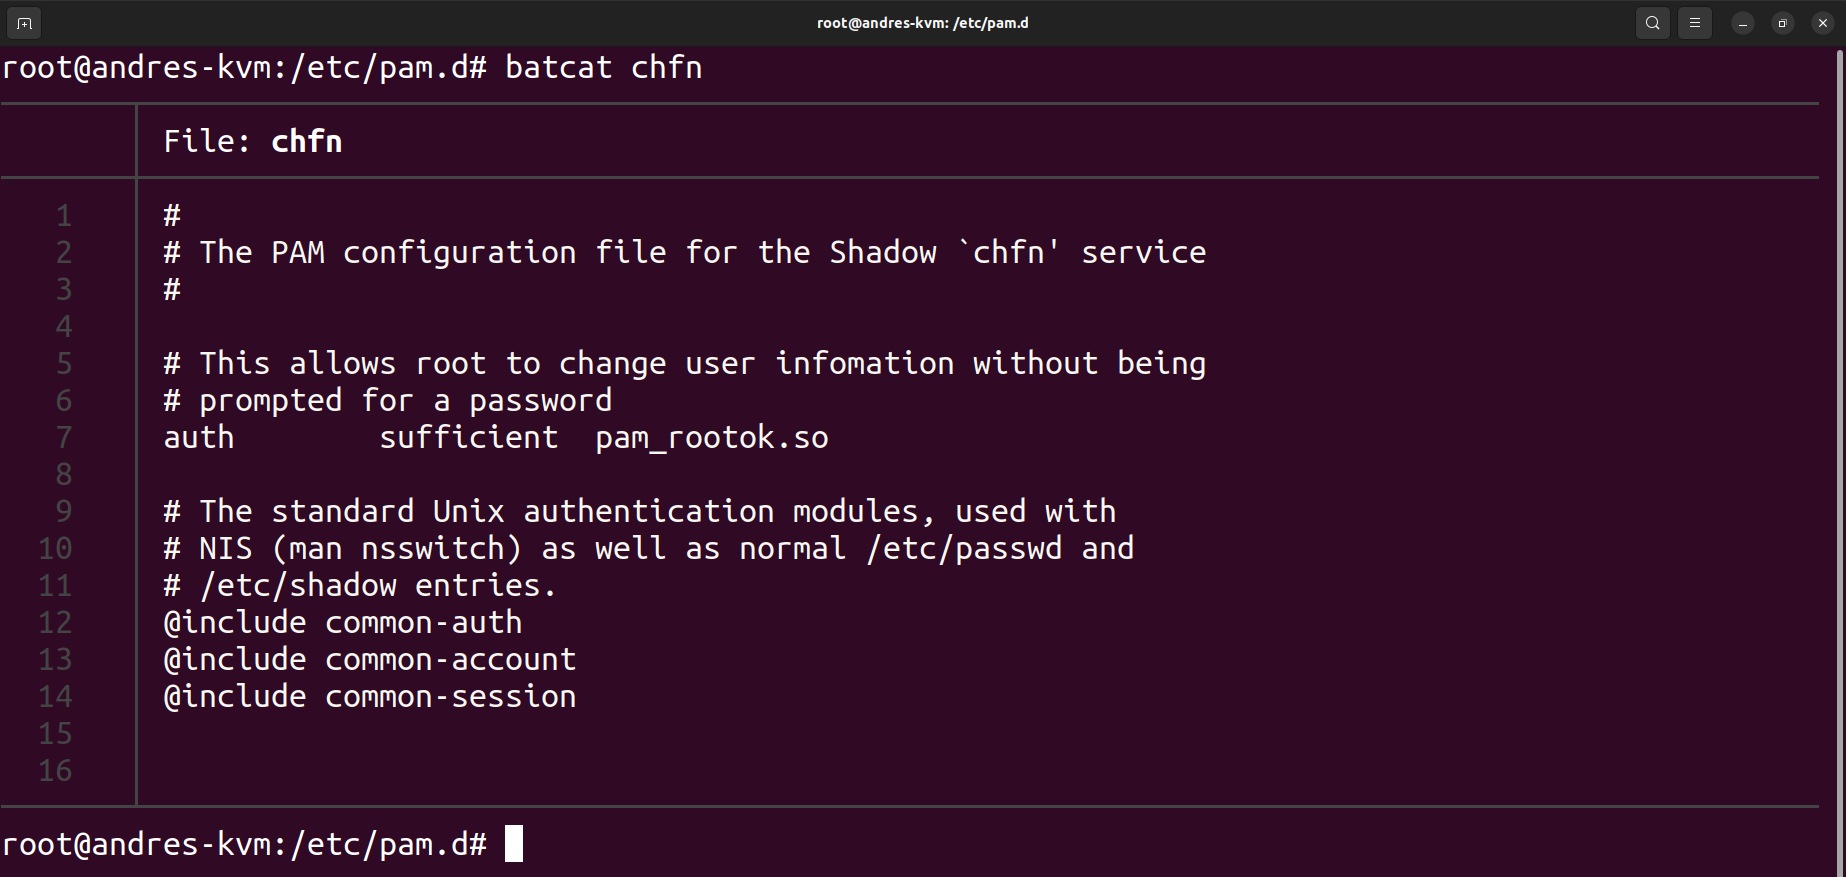
\includegraphics[width=\textwidth]{imagenes/pamchfn.png}
\end{figure}

La función de la línea 7 es para no pedir la contraseña al usuario root cuando esté usando este comando. Para ello, hace uso del campo de control sufficient, que hace que si tiene éxito retorne sin ejecutar más módulos. Además, hace uso del módulo ``pam\_rootok.so'' que hace que solo tenga éxito si el usuario tiene el UID a 0 (es el usuario root).

\addcontentsline{toc}{subsection}{/etc/pam.d/chsh}
\subsection*{/etc/pam.d/chsh}
El comando ``chsh'' permite cambiar la shell por defecto del usuario que lo invoca. Si no se le pasa ningún parámetro se activa el modo interactivo para realizar el cambio de shell.

El contenido del archivo es el siguiente:

\begin{figure}[H]
    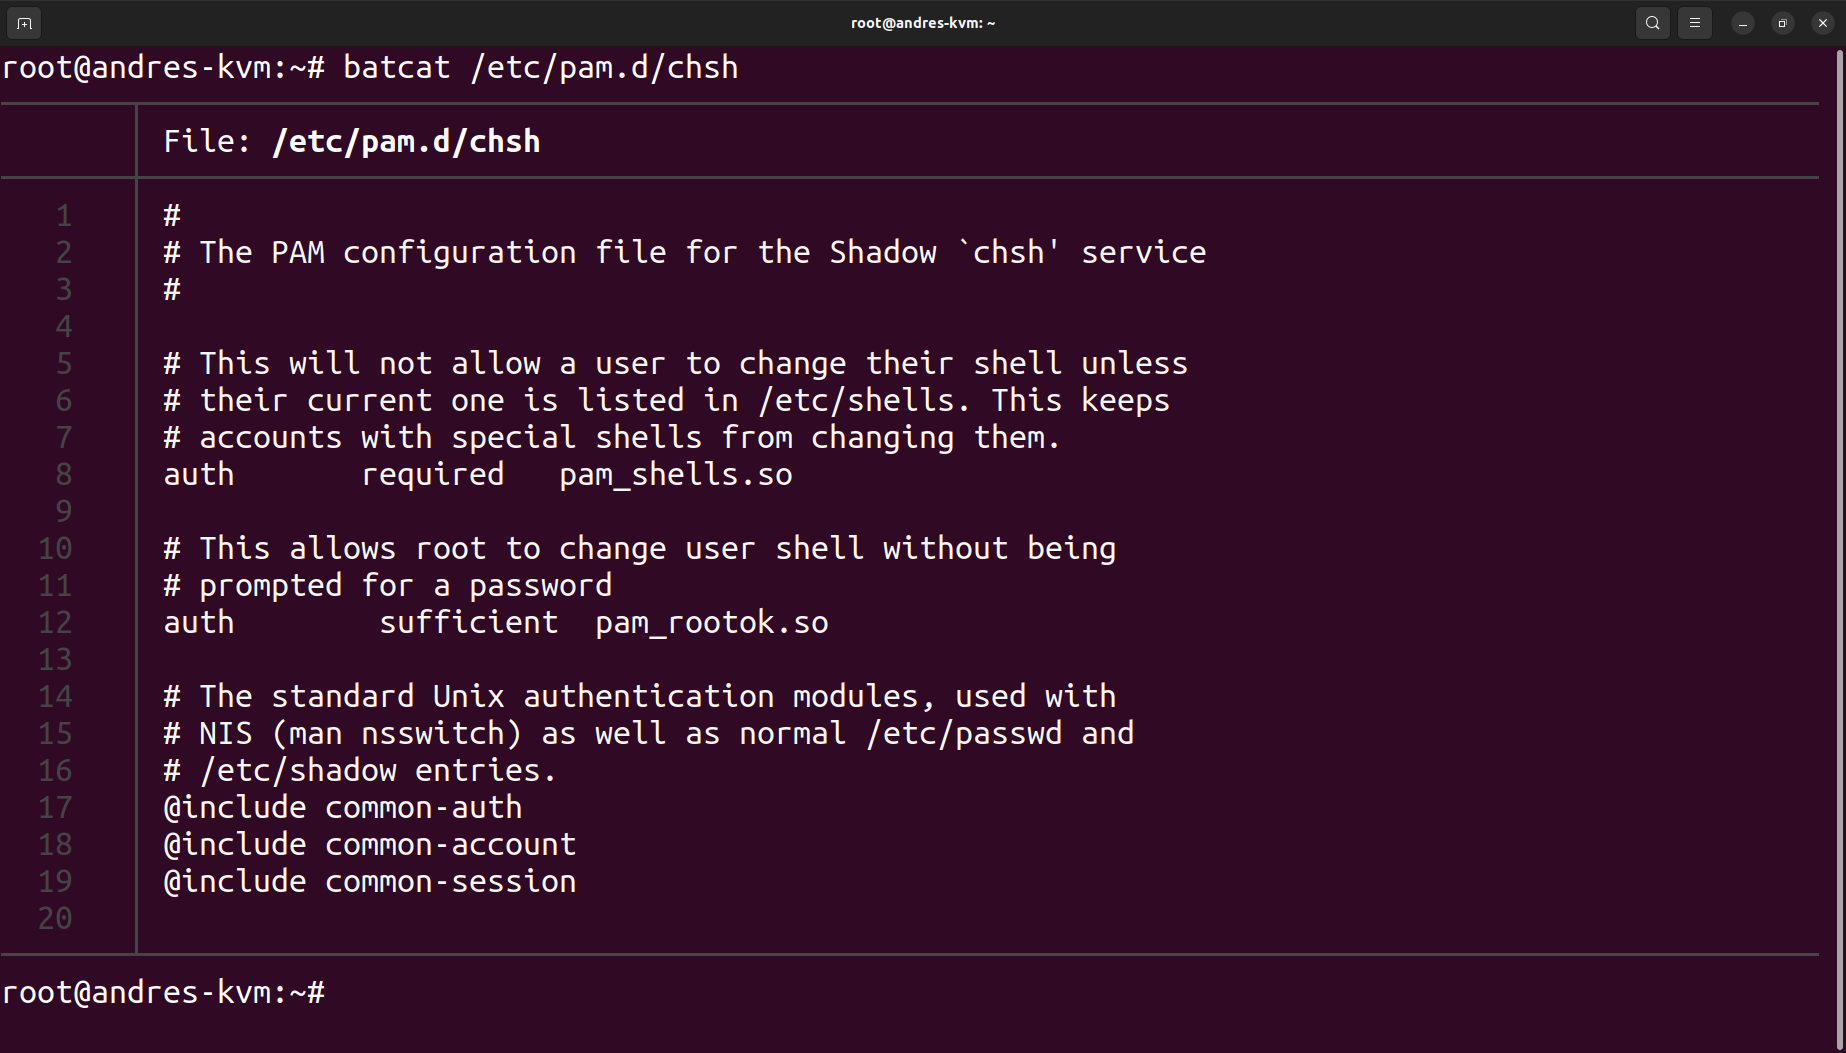
\includegraphics[width=\textwidth]{imagenes/pamchsh.png}
\end{figure}


Como se puede ver en la línea 8, esta llamada lo que hace es prohibir el cambio de shell a no ser que se encuentre listada en ``/etc/shells''. Esto se consigue mediante el campo de control ``required'', que provocará un fallo de autenticación en el sistema (ejecutará la línea siguiente, pero al ser irrelevante, no pasa nada) si el módulo falla. También se consigue mediante la llamada al módulo ``pam\_shells.so'', que hace que si la shell pasada como parámetro no se encuentra en ``/etc/shells'' dé un fallo.

La función de la línea 12 es de permitir al superusuario cambiar la shell sin ser necesario introducir la contraseña. Esto se realiza mediante el campo de control ``sufficient'' y el módulo ``pam\_rootok.so''. Con ``sufficient'', cuando la orden tiene éxito retorna sin ejecutar los demás módulos. Además, con el módulo ``pam\_rootok.so'' autoriza al usuario con el UID 0 (root).


\addcontentsline{toc}{section}{Ejercicio 5}
\section*{Ejercicio 5}
\addcontentsline{toc}{subsection}{Apartado A}
\subsection*{Apartado A}
Es necesario modificar el archivo PAM ``common-password'' y en Ubuntu 22.04 ya como primera línea aparece el uso del módulo ``pam\_pwquality''. 

Ahora bien si leemos el manual de este módulo con ``man 8 pam\_pwquality'' se puede ver que hay un argumento denominado ``minlen'' y que valor por defecto es 8. No obstante, no se puede bajar del valor 4, ya que es un límite que tiene ``Cracklib'' y mostrara que la contraseña es muy corta. Por eso, voy a poner el límite a \textbf{15 caracteres}.

\begin{figure}[H]
    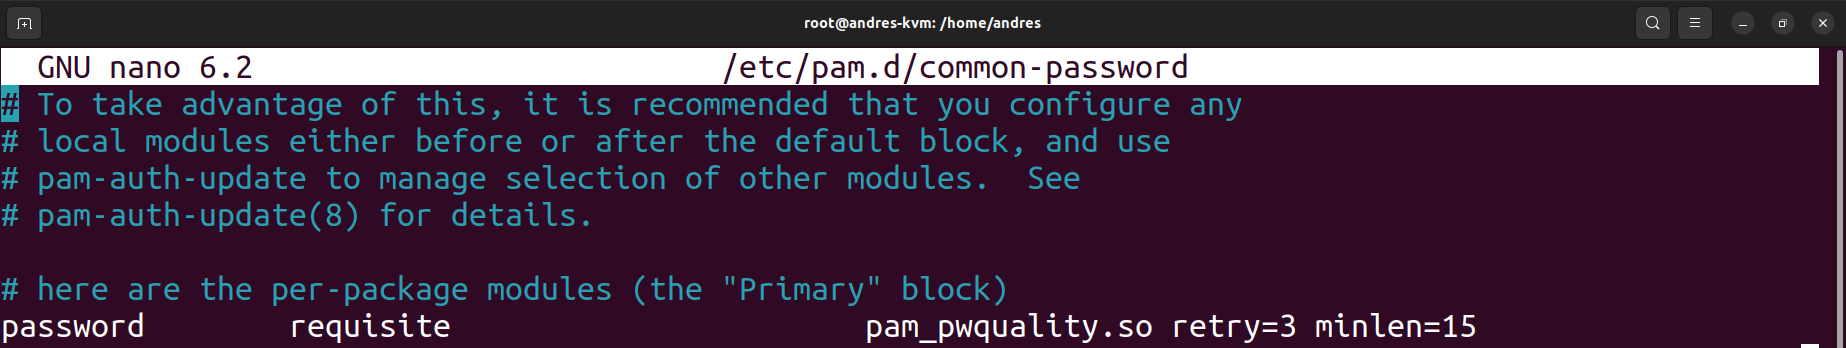
\includegraphics[width=\textwidth]{imagenes/passwordminlen15.png}
\end{figure}

Y ahora al usar el comando ``passwd'' y poner una contraseña con menos de 15 palabras, muestra un error:

\begin{figure}[H]
    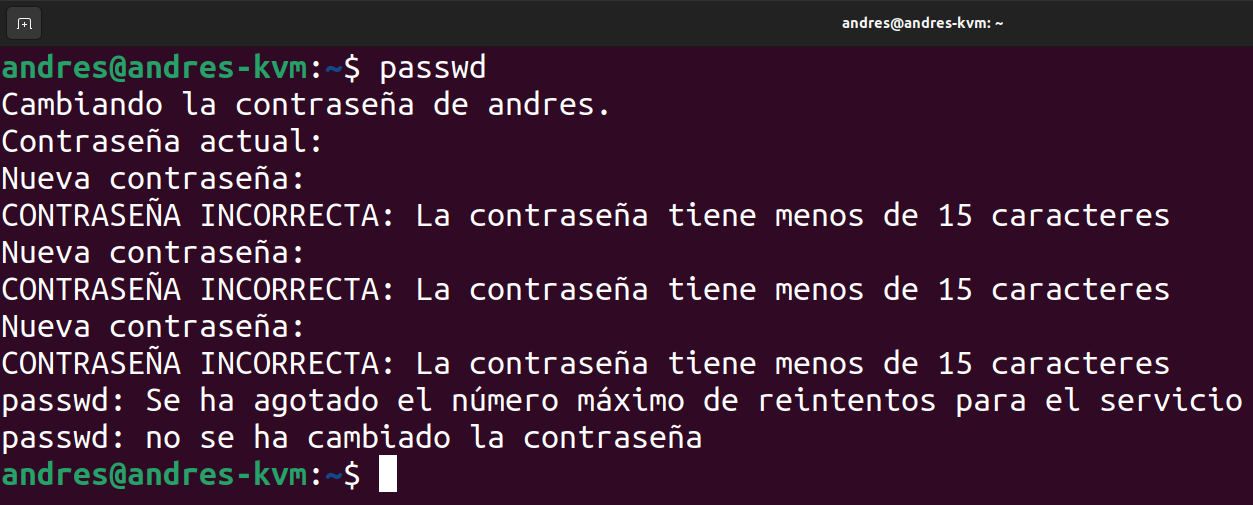
\includegraphics[width=\textwidth]{imagenes/passwordminlen15passwd.png}
\end{figure}

Y al agotarse los intentos (que son 3) se sale del programa.
\addcontentsline{toc}{subsection}{Apartado B}
\subsection*{Apartado B}
En esta parte he restringido el acceso al comando ``su'' para así evitar que un usuario que ponga el comando sin ``sudo'' pueda entrar. Si ponen ``sudo su'' sí van a poder entrar, pero esto es así, ya que son usuarios administradores (y es una decisión de diseño, ya que en otro caso no podría usar nadie ``sudo''), en ese caso lo recomendable es deshabilitar el acceso al grupo ``sudo'' (en el caso de Ubuntu) para que no lo pueda usar (editando el archivo sudoers mediante el comando ``visudo'').

Para conseguir esto, es necesario modificar el archivo ``/etc/pam.d/su'' y añadir la siguiente línea al principio:

\begin{figure}[H]
    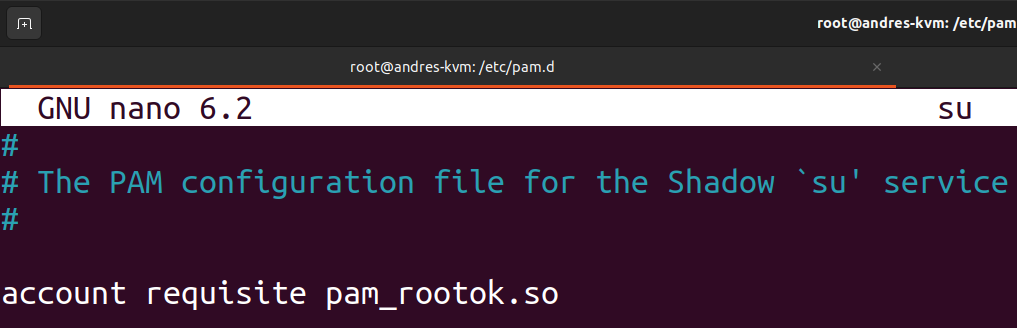
\includegraphics[width=\textwidth]{imagenes/sudeny.png}
\end{figure}

Ahora, al ejecutar el comando ``su'' con un usuario normal aparece lo siguiente:

\begin{figure}[H]
    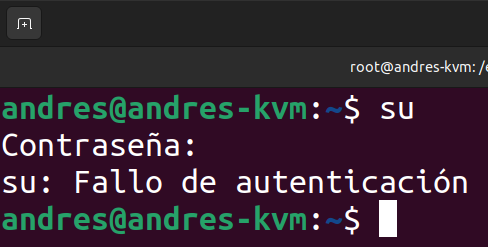
\includegraphics[width=\textwidth]{imagenes/sudenyuser.png}
\end{figure}


En cambio, si el usuario puede usar ``sudo'', si puede acceder.

\begin{figure}[H]
    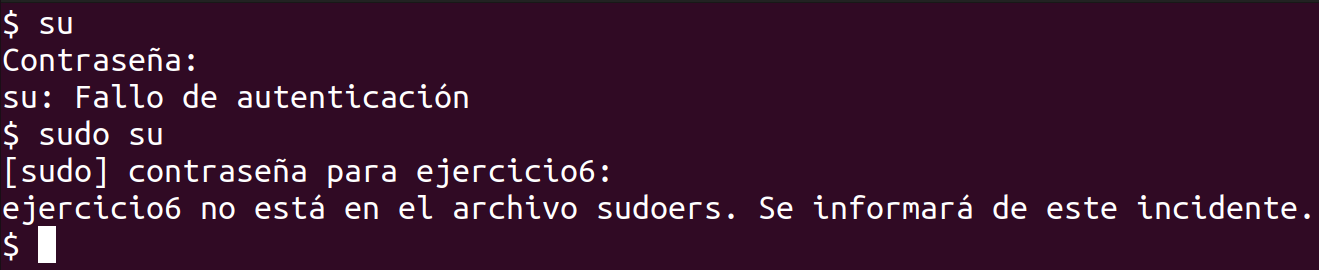
\includegraphics[width=\textwidth]{imagenes/sudenyuserprueba.png}
    \caption{El usuario que se ha creado en esta práctica no tiene permisos para usar ``sudo'' y por tanto no puede entrar de ninguna manera}
\end{figure}

La línea que he añadido lo que hace es comprobar que la cuenta sea root (UID=0) y en caso de no serlo, no sigue ejecutando el archivo provocando un error de autenticación.


\addcontentsline{toc}{section}{Ejercicio 6}
\section*{Ejercicio 6}
En Ubuntu 22.04 los cambios de contraseña no se almacenan en ``/var/log/messages'', sino en ``/var/log/auth.log''. \href{https://ubuntu.com/tutorials/viewing-and-monitoring-log-files#2-log-files-locations}{Enlace} a la guía.


Voy a crear el usuario ``ejercicio6'' y le voy a cambiar la contraseña:

\begin{figure}[H]
    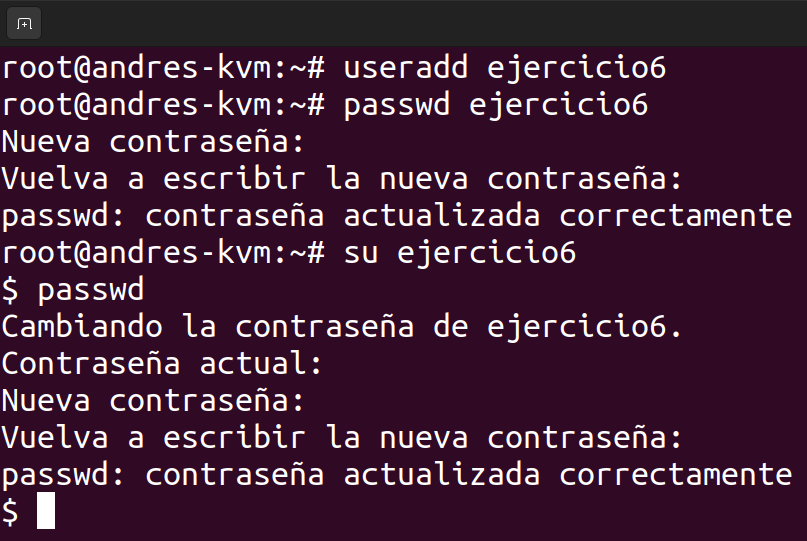
\includegraphics[width=\textwidth]{imagenes/createejercicio6.png}
\end{figure}

Y ahora, al mostrar el archivo ``/var/log/auth.log'' aparecen las siguientes líneas:

\begin{figure}[H]
    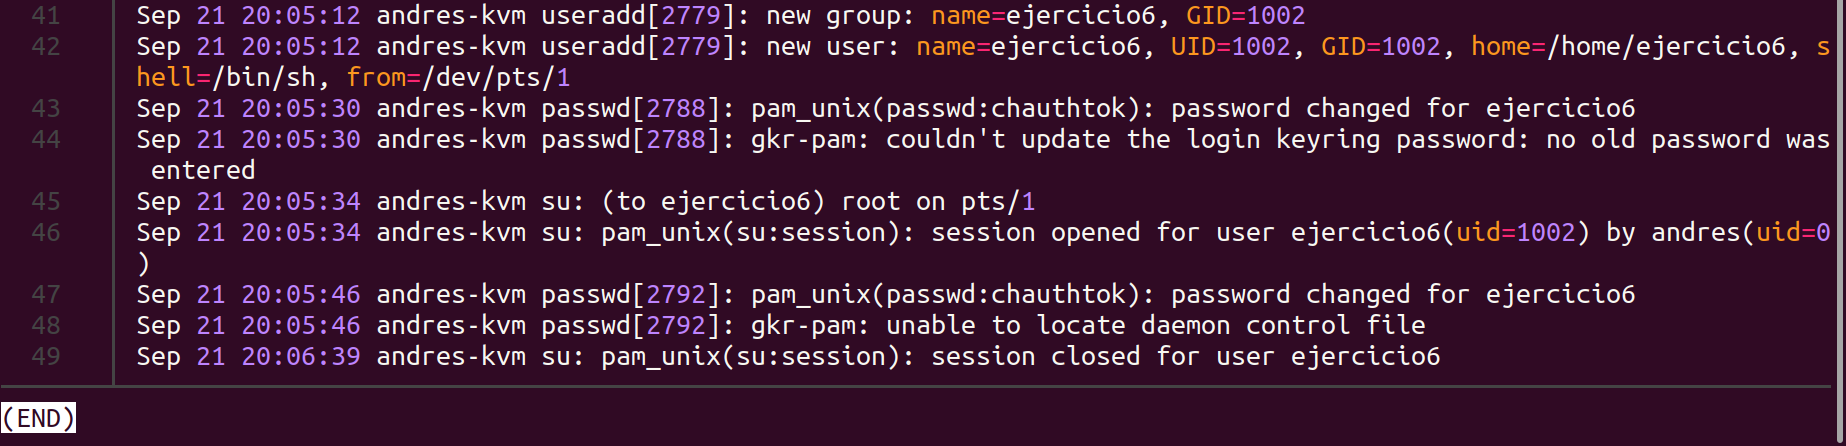
\includegraphics[width=\textwidth]{imagenes/authcreateejercicio6.png}
\end{figure}

\addcontentsline{toc}{section}{Ejercicio 7}
\section*{Ejercicio 7}
Para empezar, el propio archivo de sudoers recomienda usar la orden ``visudo''. POr tanto, es necesario usar ``visudo'' para que no haya problemas después. Además, por defecto usa el editor ``vi'', esto se puede cambiar usando el comando siguiente:

\verb|EDITOR=nano visudo|

Ahora, voy a asignarle permisos para usar sudo al usuario ``prueba'' que no se encuentra en el grupo ``sudo'', que es el que usa Ubuntu para dar permisos.

\begin{figure}[H]
    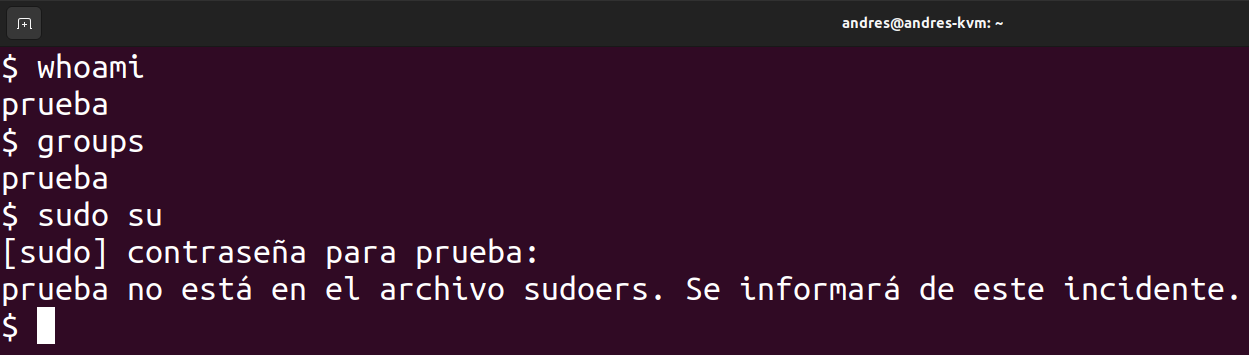
\includegraphics[width=\textwidth]{imagenes/sudoprueba.png}
\end{figure}

Si añadimos la siguiente línea en el archivo ``sudoers'' tendremos acceso con ``sudo'':

\begin{figure}[H]
    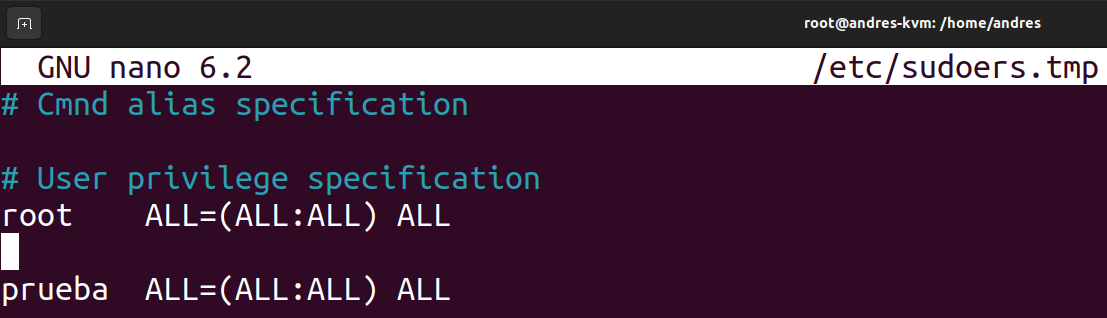
\includegraphics[width=\textwidth]{imagenes/sudoersprueba.png}
\end{figure}


Y ahora al hacer una prueba se puede ver que ya funciona:

\begin{figure}[H]
    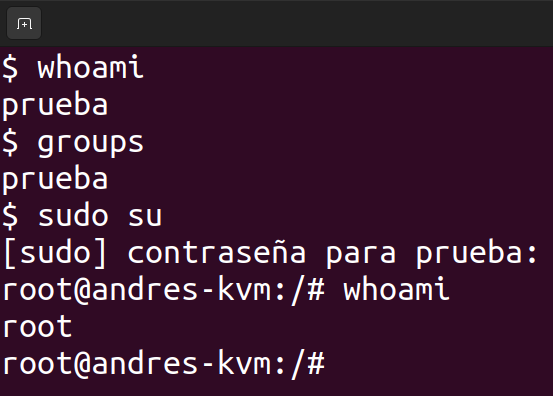
\includegraphics[width=\textwidth]{imagenes/sudopruebaok.png}
\end{figure}

\addcontentsline{toc}{section}{Ejercicio 8}
\section*{Ejercicio 8}
Voy a examinar cada uno de los archivos y comprobar que se registran eventos que realizaré. Para ello, voy a dividir la explicación en subsecciones para cada uno de los archivos.

\addcontentsline{toc}{subsection}{/var/log/lastlog}
\subsection*{/var/log/lastlog}
Este archivo almacena información sobre le ultimo inicio de sesión de los usuarios. Para acceder a la información es necesario utilizar el comando ``lastlog'':

\begin{figure}[H]
    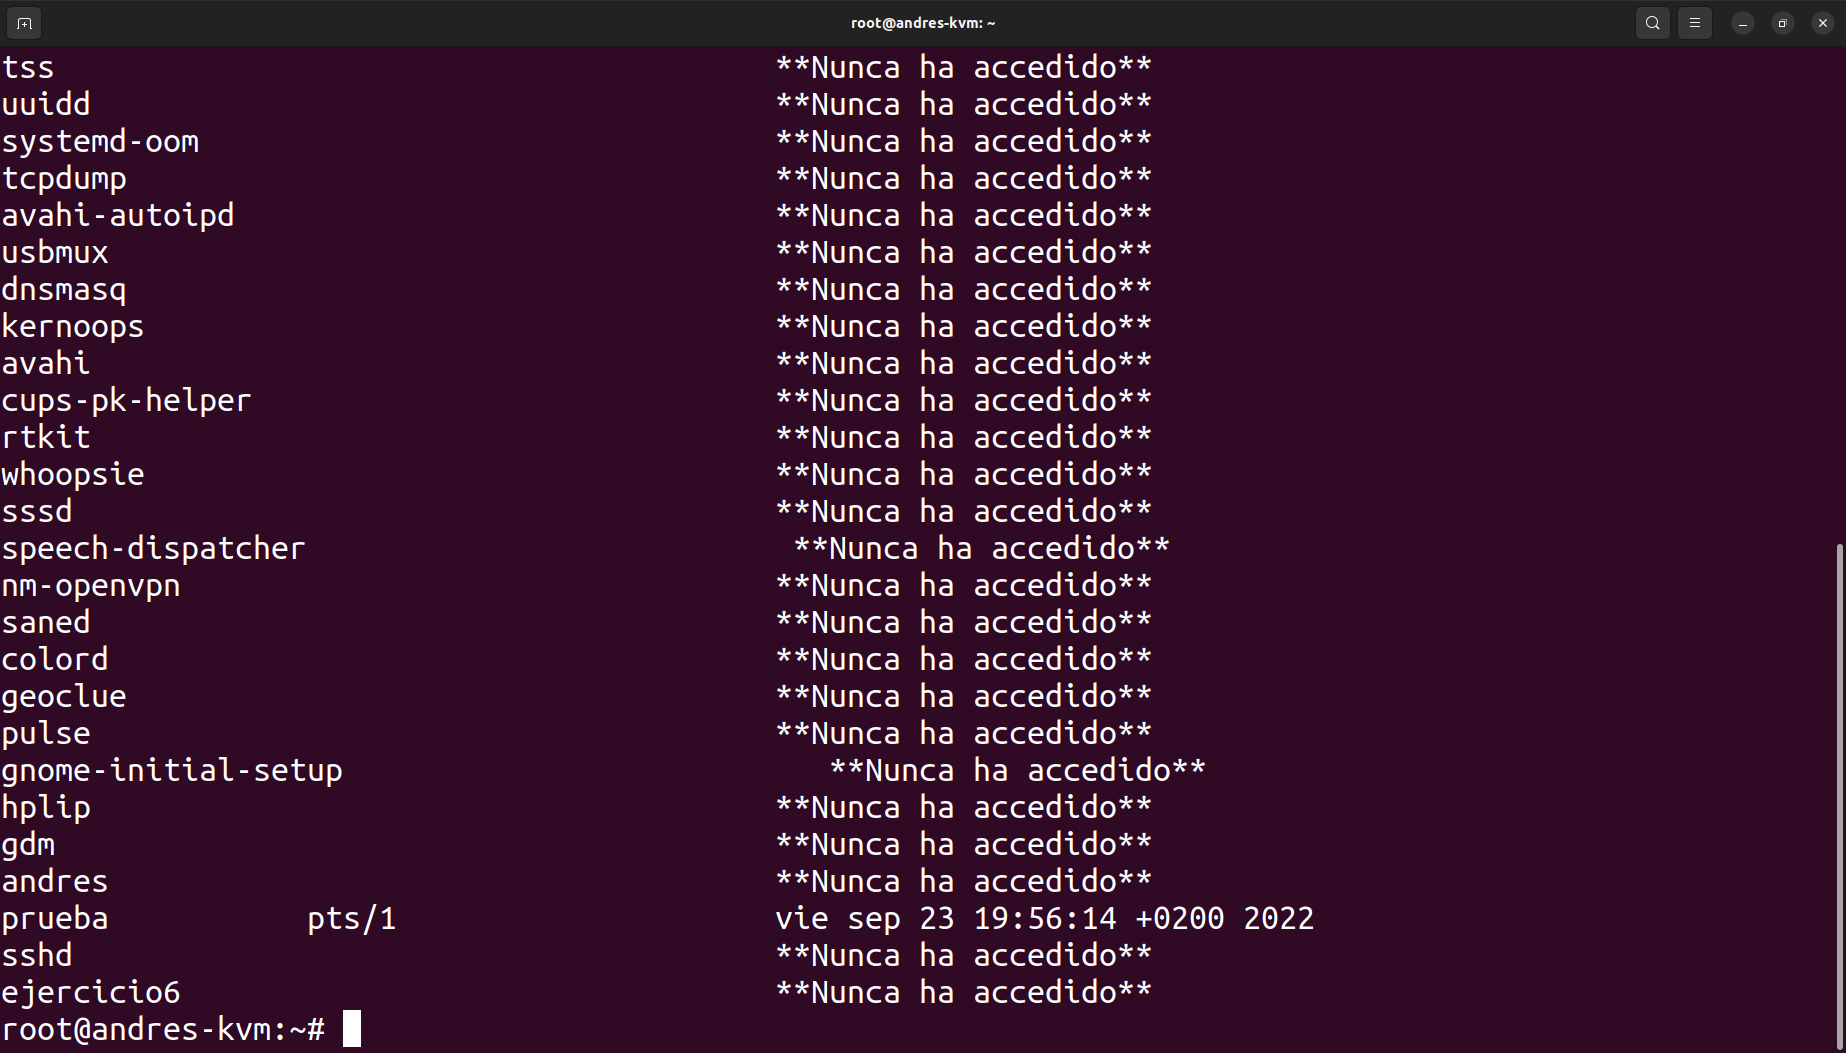
\includegraphics[width=\textwidth]{imagenes/lastlogejercicio6never.png}
\end{figure}

Como se puede ver, el usuario ``ejercicio6'' nunca ha iniciado sesión en el sistema. Ahora si inicio sesión y vuelvo a usar la orden ``lastlog'' aparece lo siguiente:

\begin{figure}[H]
    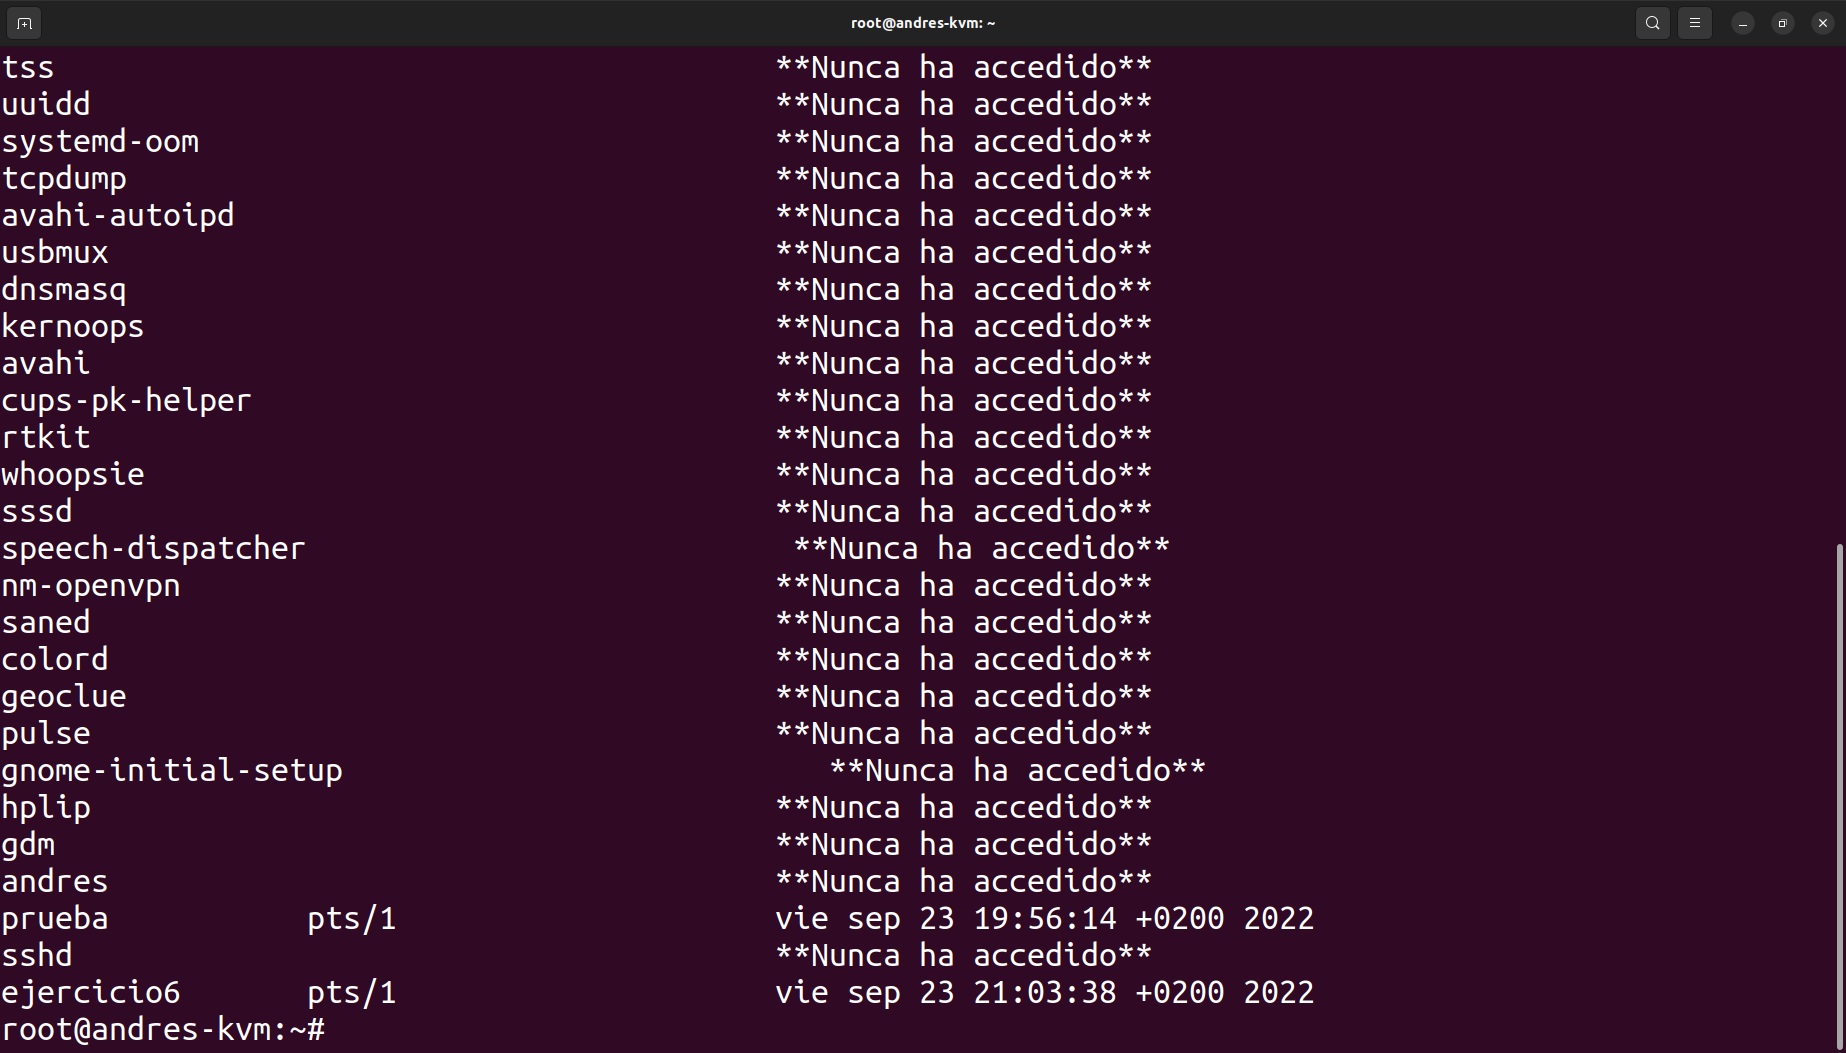
\includegraphics[width=\textwidth]{imagenes/lastlogejercicio6ok.png}
\end{figure}

Ahora como se puede ver aparece la fecha del último inicio de sesión del usuario ``ejercicio6''.

\addcontentsline{toc}{subsection}{/var/log/wtmp}
\subsection*{/var/log/wtmp}
Almacena los login y logout de los distintos usuarios del sistema. Se accede con el comando ``last''. 

\begin{figure}[H]
    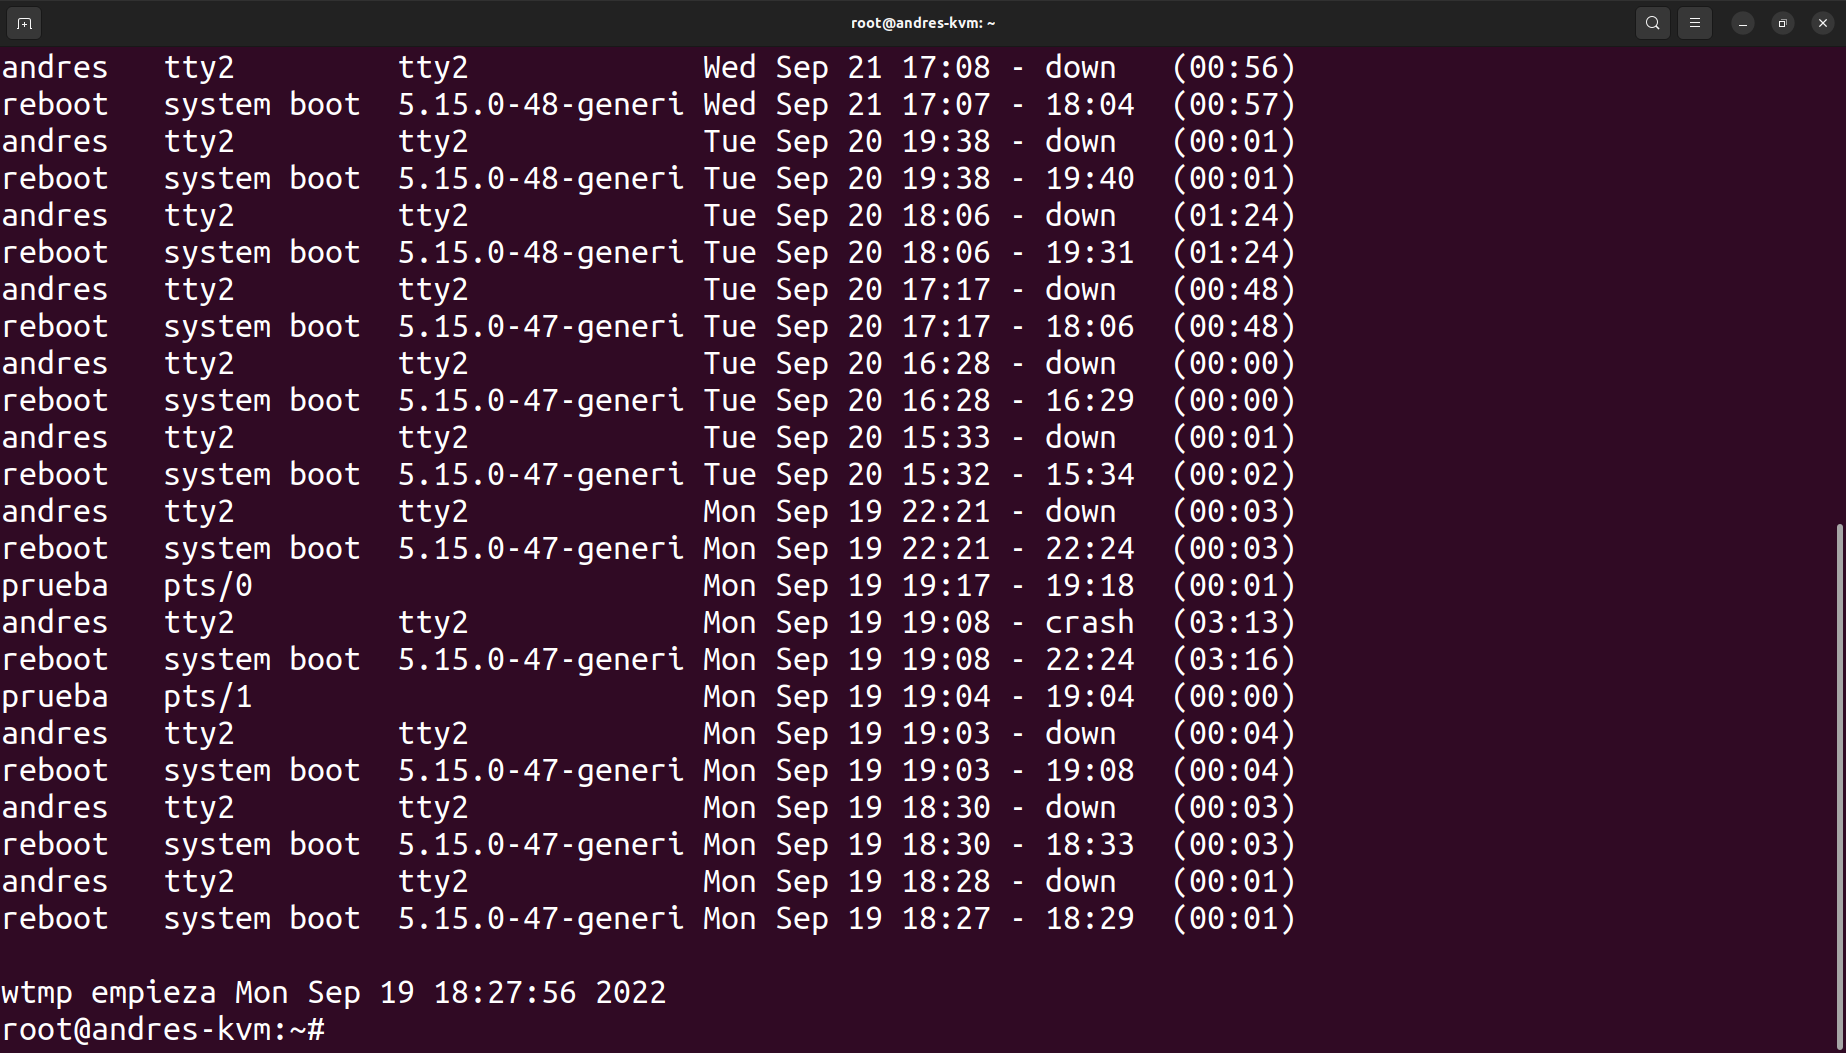
\includegraphics[width=\textwidth]{imagenes/lastnormal.png}
\end{figure}

Ahora con el comando ``last --since today'' muestra solo la información de hoy.

\begin{figure}[H]
    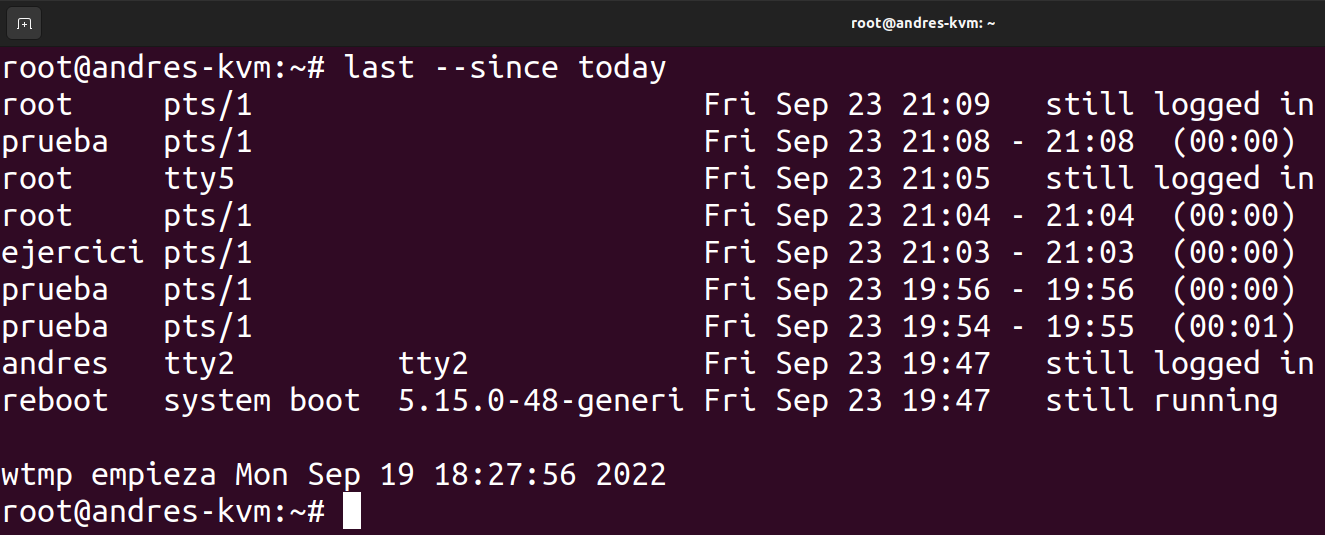
\includegraphics[width=\textwidth]{imagenes/lasttoday.png}
\end{figure}

Y ahora voy a iniciar sesión con el usuario ``prueba'' y logout para ver como se almacena la información:

\begin{figure}[H]
    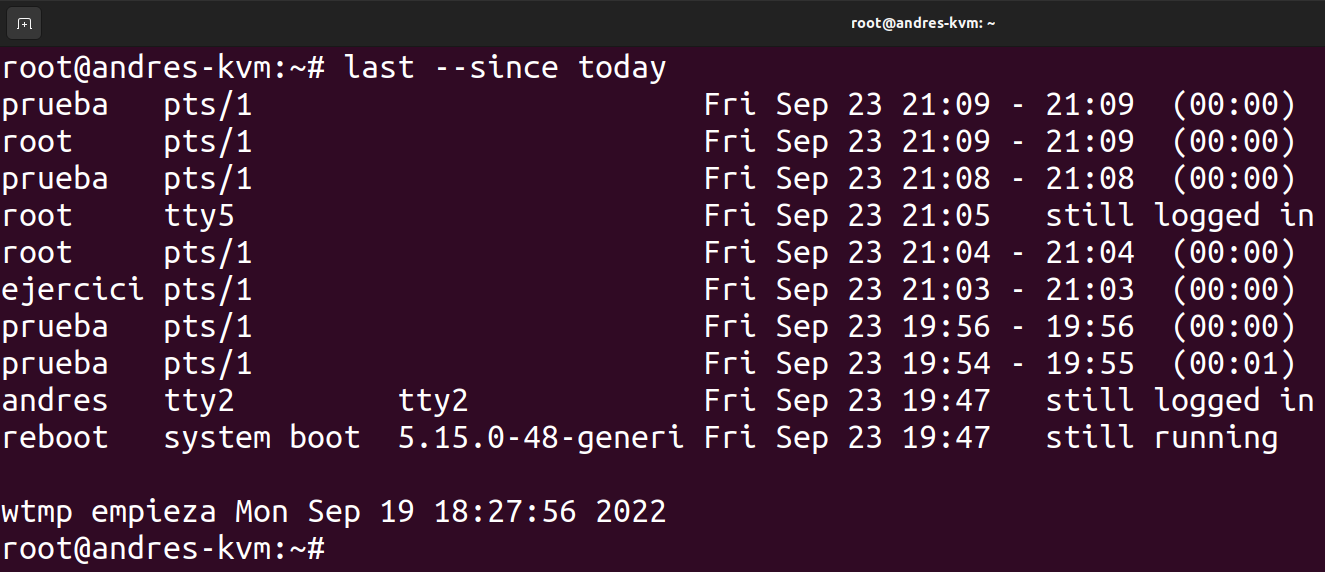
\includegraphics[width=\textwidth]{imagenes/lasttodayprueba.png}
\end{figure}

\addcontentsline{toc}{subsection}{/var/log/utmp}
\subsection*{/var/log/utmp}
Muestra los usuarios que están \textit{loggeados} en el sistema. Se puede obtener esta información con la orden ``who''.

\begin{figure}[H]
    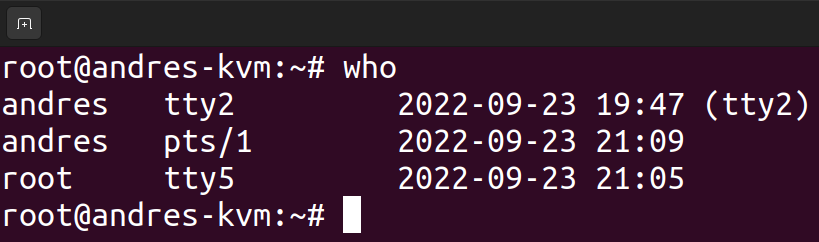
\includegraphics[width=\textwidth]{imagenes/whonormal.png}
\end{figure}

Ahora si inicio sesión con el usuario ``prueba'' debería aparecer con el comando anterior:

\begin{figure}[H]
    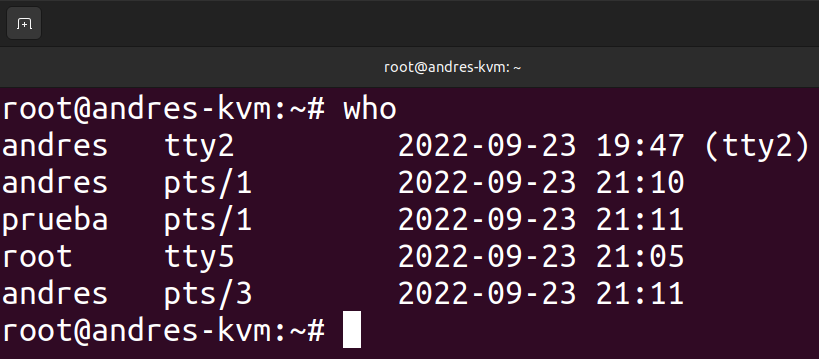
\includegraphics[width=\textwidth]{imagenes/whoprueba.png}
\end{figure}

\addcontentsline{toc}{subsection}{/var/log/btmp}
\subsection*{/var/log/btmp}
Muestra los intentos fallidos de inicio de sesión en el sistema. Se puede obtener con la orden ``lastb''.

\begin{figure}[H]
    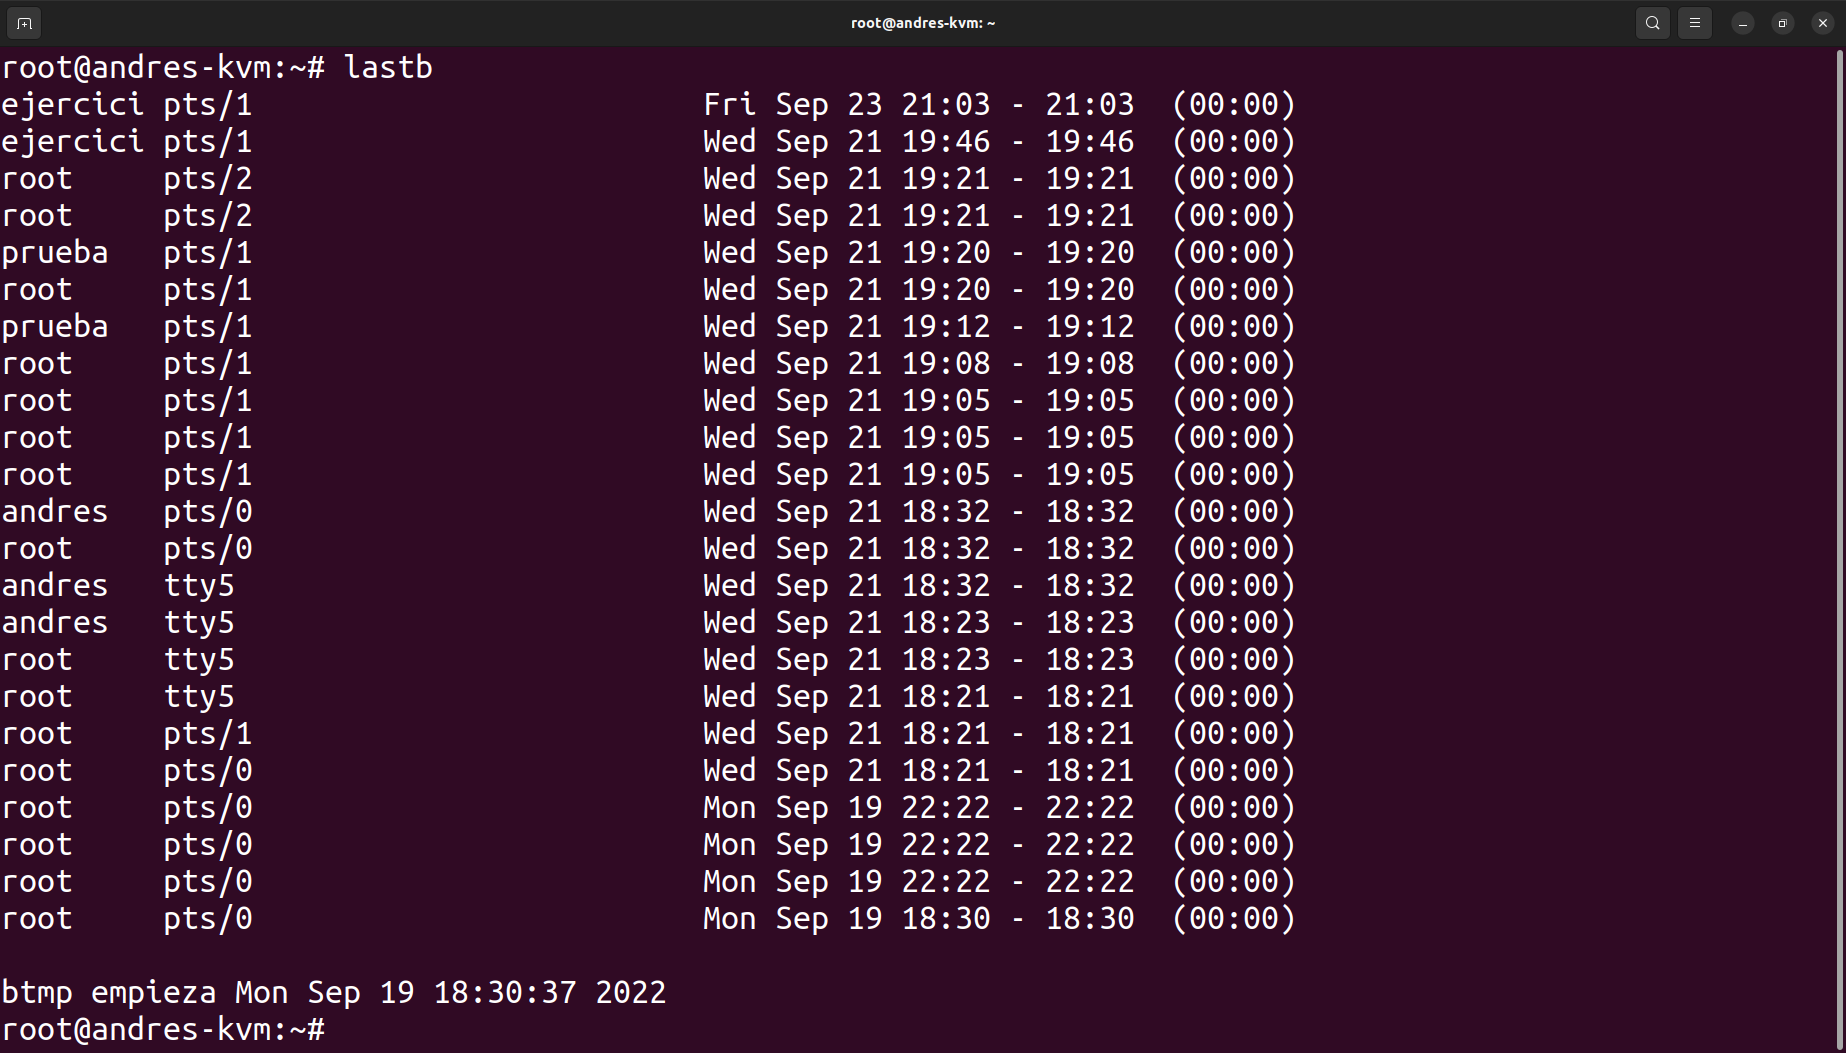
\includegraphics[width=\textwidth]{imagenes/lastbnormal.png}
\end{figure}

Ahora, si hago que fallo el inicio de sesión del usuario ``prueba'' debería de salir:

\begin{figure}[H]
    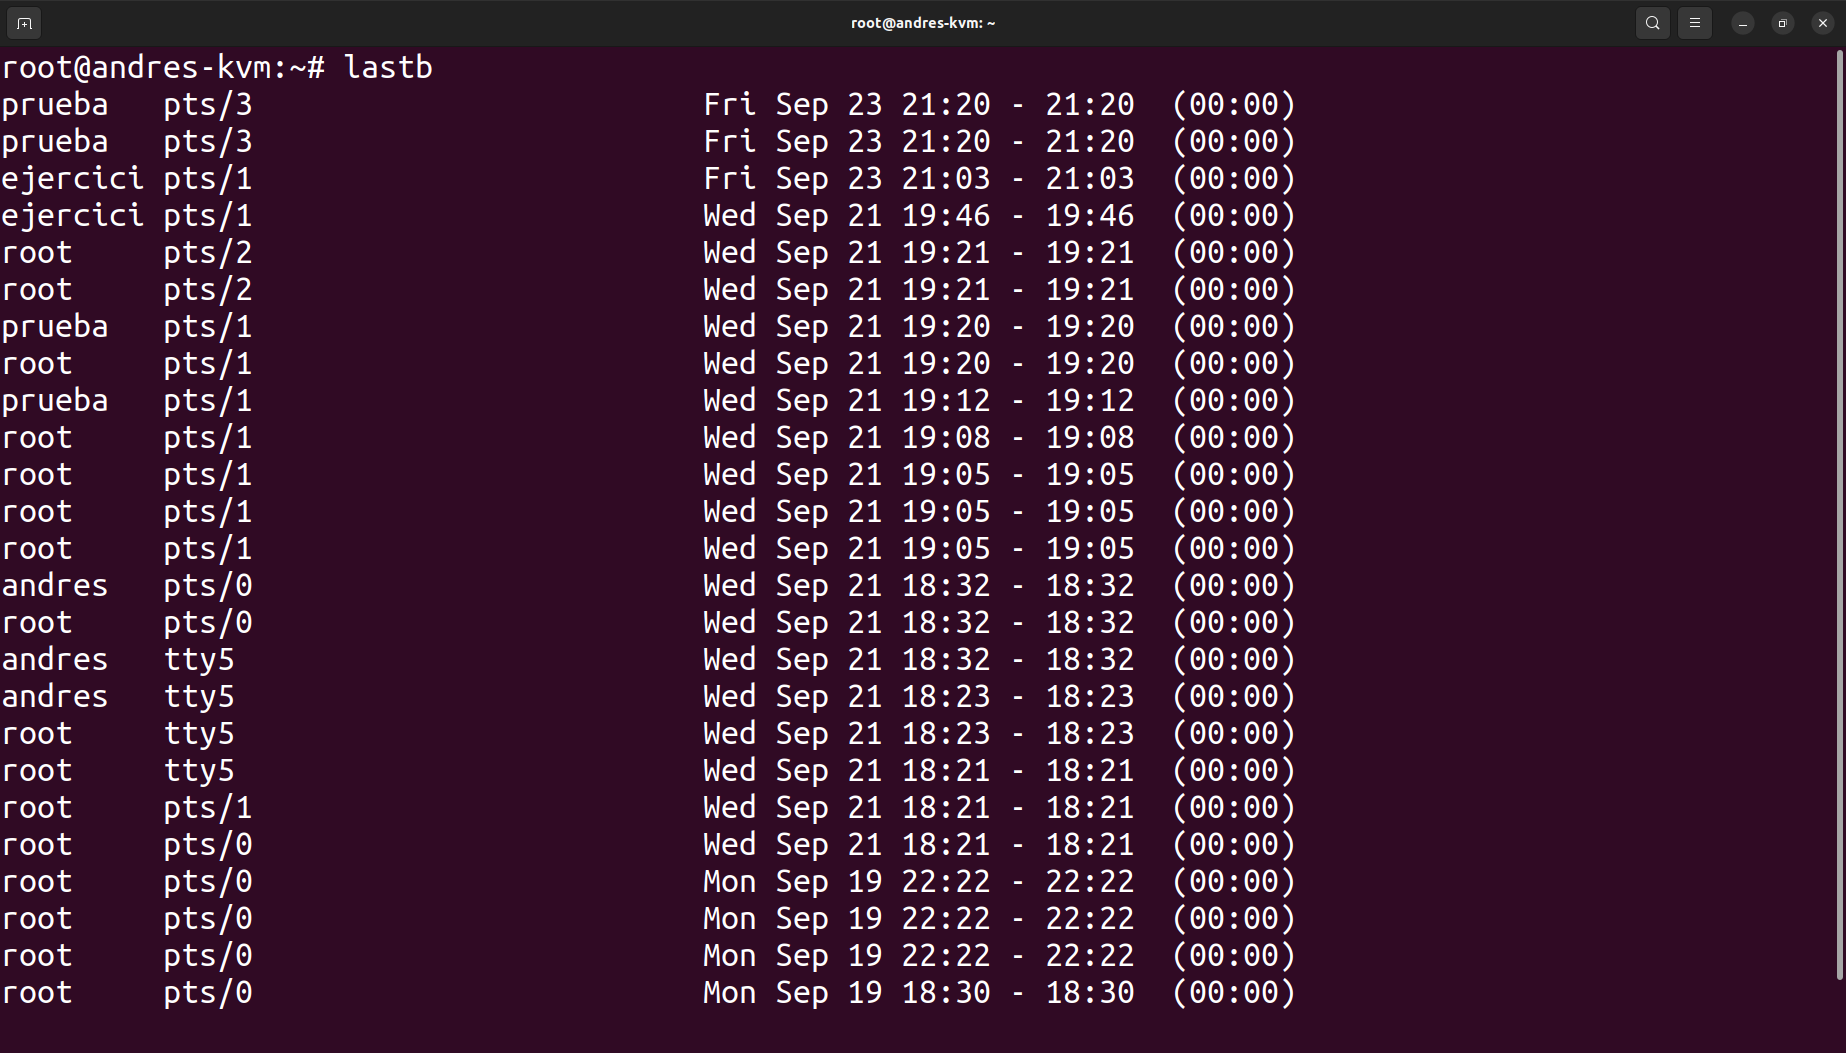
\includegraphics[width=\textwidth]{imagenes/lastbpruebafirst.png}
    \caption{Se puede ver que las dos primeras líneas pertenecen a intentos de login con el usuario ``prueba''.}
\end{figure}

\addcontentsline{toc}{subsection}{/var/log/sudo}
\subsection*{/var/log/sudo}
Este archivo, al menos en Ubuntu, no existe, por tanto no puedo mostrar información al respecto sobre la actividad del uso de ``sudo''.

\addcontentsline{toc}{subsection}{/var/log/messages}
\subsection*{/var/log/messages}
En Ubuntu (no sé si en otras distribuciones también) ya no existe este archivo porque duplicaba información con ``/var/log/syslog''. Por tanto, voy a mostrar este archivo:

\begin{figure}[H]
    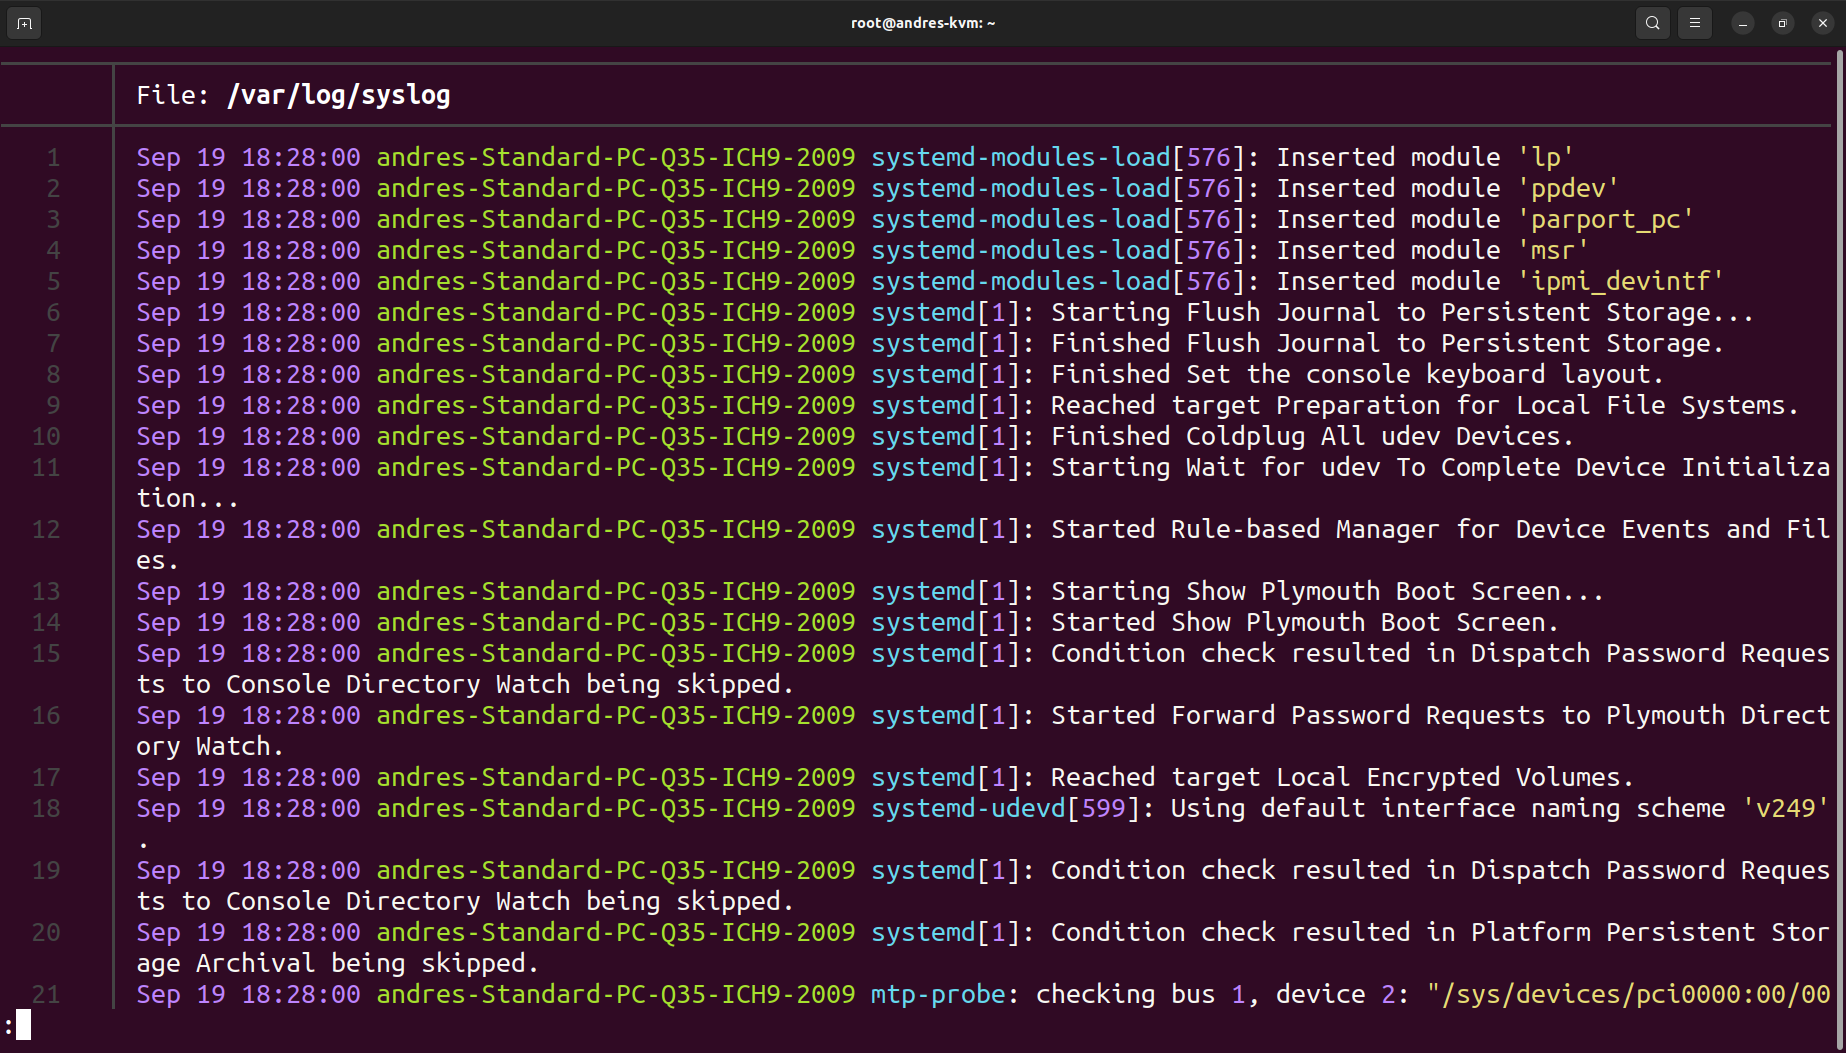
\includegraphics[width=\textwidth]{imagenes/syslog.png}
\end{figure}

\addcontentsline{toc}{section}{Ejercicio 9}
\section*{Ejercicio 9}

\addcontentsline{toc}{subsection}{PC de mi casa}
\subsection*{PC de mi casa}
Para comprobar los intentos de inicio de sesión fallidos en el ordenador de mi casa, voy a usar ``lastb'':

\begin{figure}[H]
    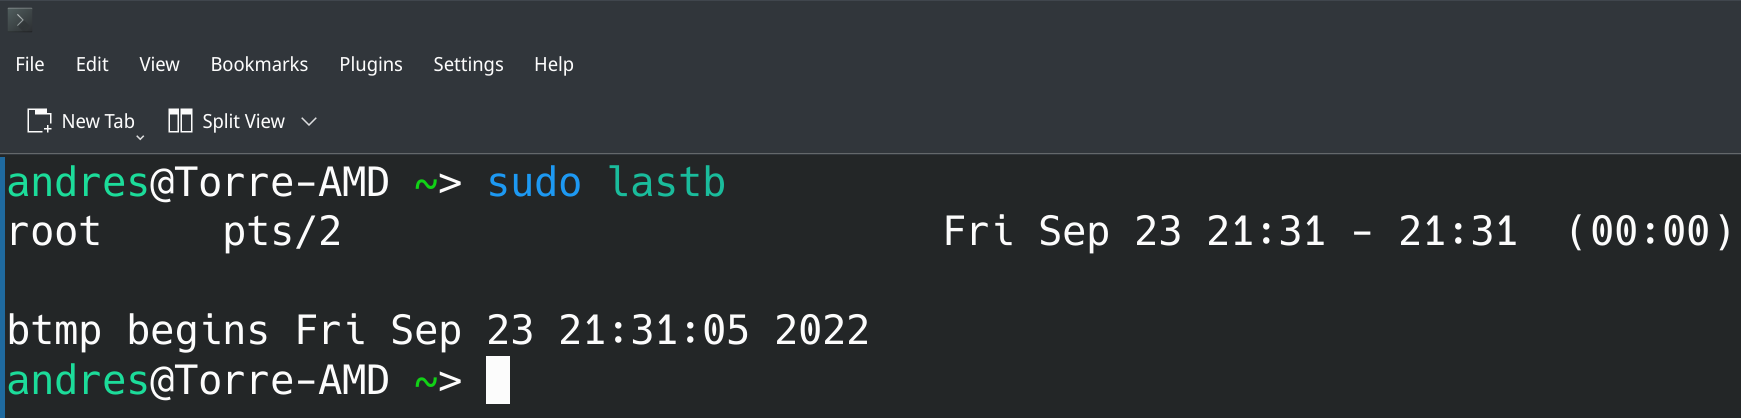
\includegraphics[width=\textwidth]{imagenes/lastbcasa.png}
\end{figure}

Como se puede observar, el único intento fallido de inicio de sesión que he tenido ha sido provocado por mí en el momento de hacer esta parte del ejercicio.

Ahora, muestro con el comando ``last'' los login y logout del sistema:

\begin{figure}[H]
    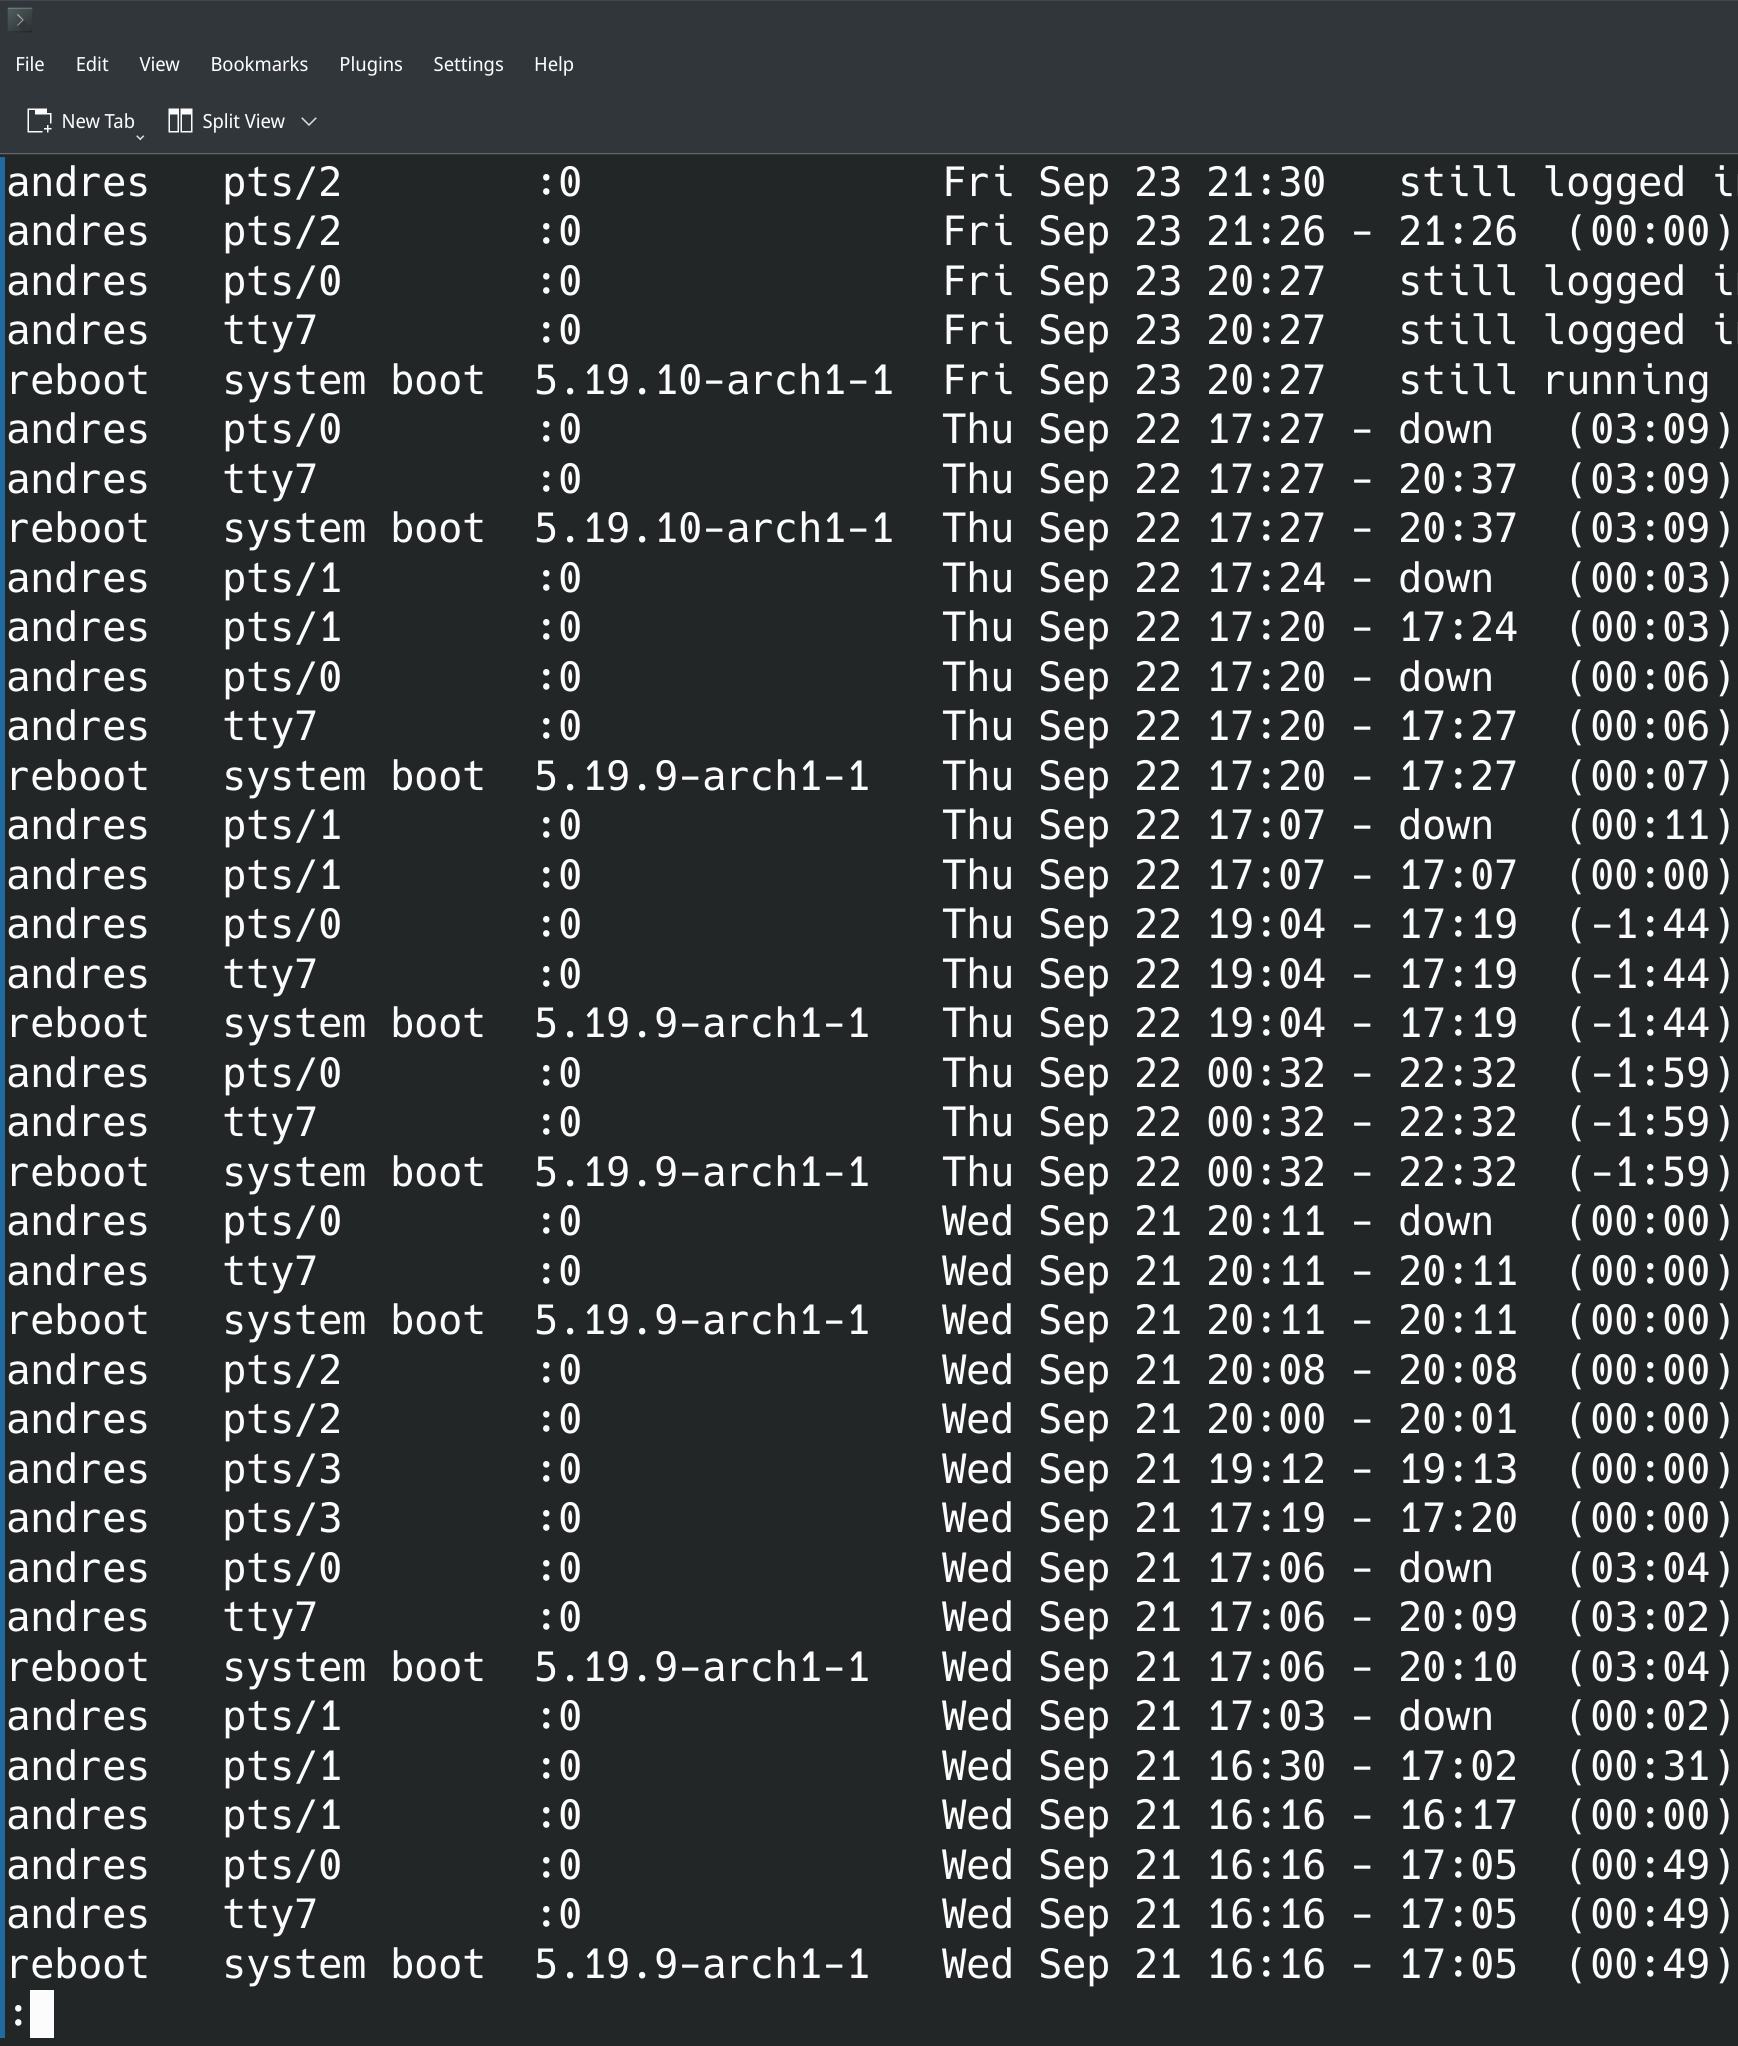
\includegraphics[width=\textwidth]{imagenes/lastcasa.png}
\end{figure}

Por lo que puedo ver, no ha habido ningún inicio en el sistema por SSH (se mostraría en la tercera columna la dirección IP del que lo ha intentado).

Por último, con la orden ``lastlog'' muestro los inicios de sesión producidos en el sistema.

\begin{figure}[H]
    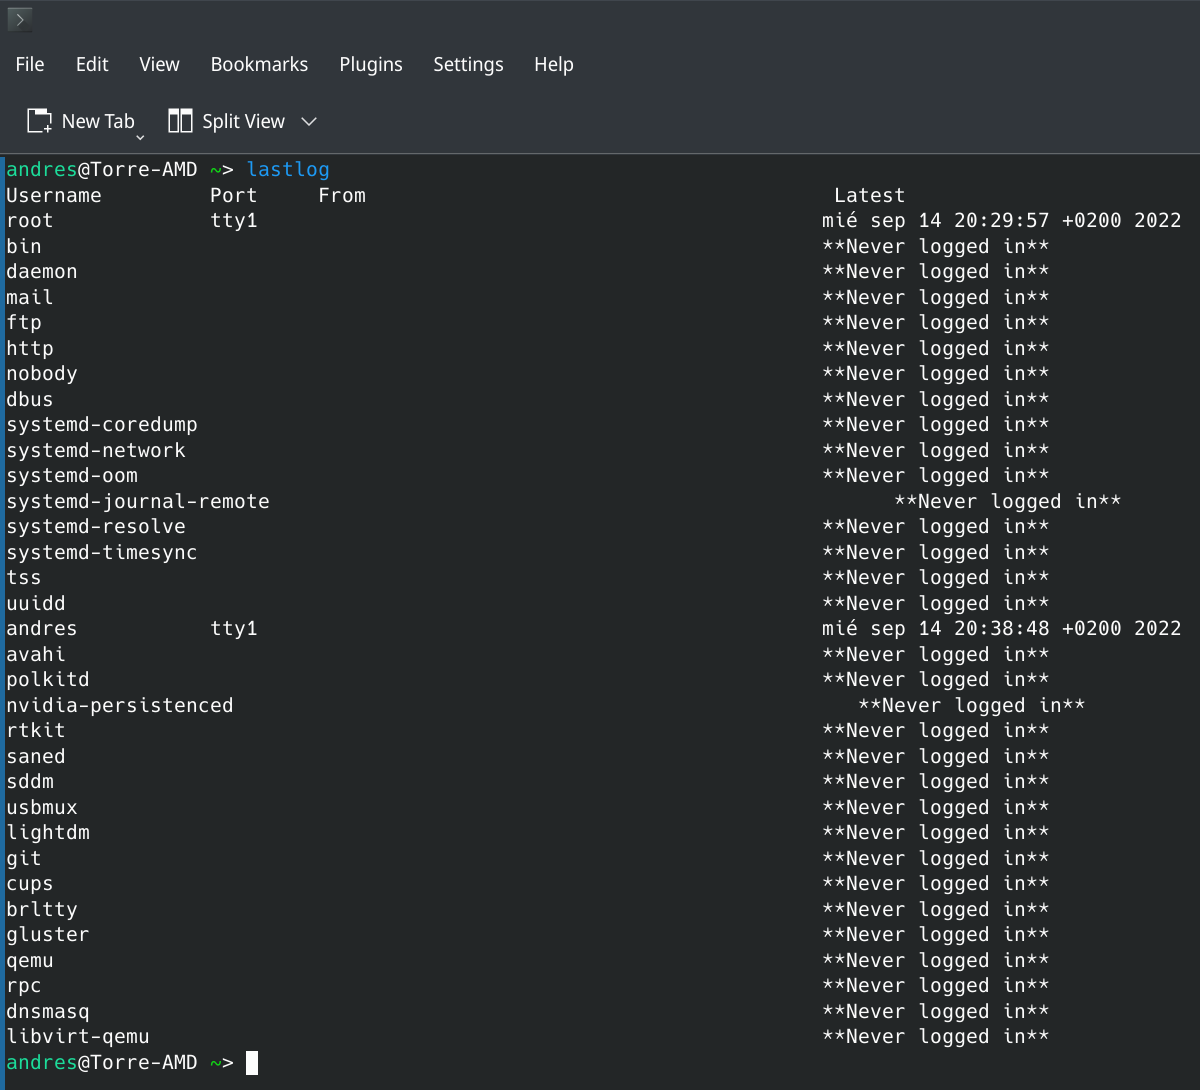
\includegraphics[width=\textwidth]{imagenes/lastlogcasa.png}
\end{figure}

Como se puede ver, no hay ninguno en el que aparezca SSH y los inicios de sesión me concuerdan, lo cual me puede indicar que el sistema no ha sido (a simple vista) comprometido.

\addcontentsline{toc}{subsection}{PC de prácticas (máquina virtual)}
\subsection*{PC de prácticas (máquina virtual)}
Voy a usar los mismos comandos para la máquina virtual y comprobar su seguridad. Para suponer que el sistema ha sido comprometido, he usado SSH desde el ordenador de mi casa (host) hacia la máquina virtual.

\begin{figure}[H]
    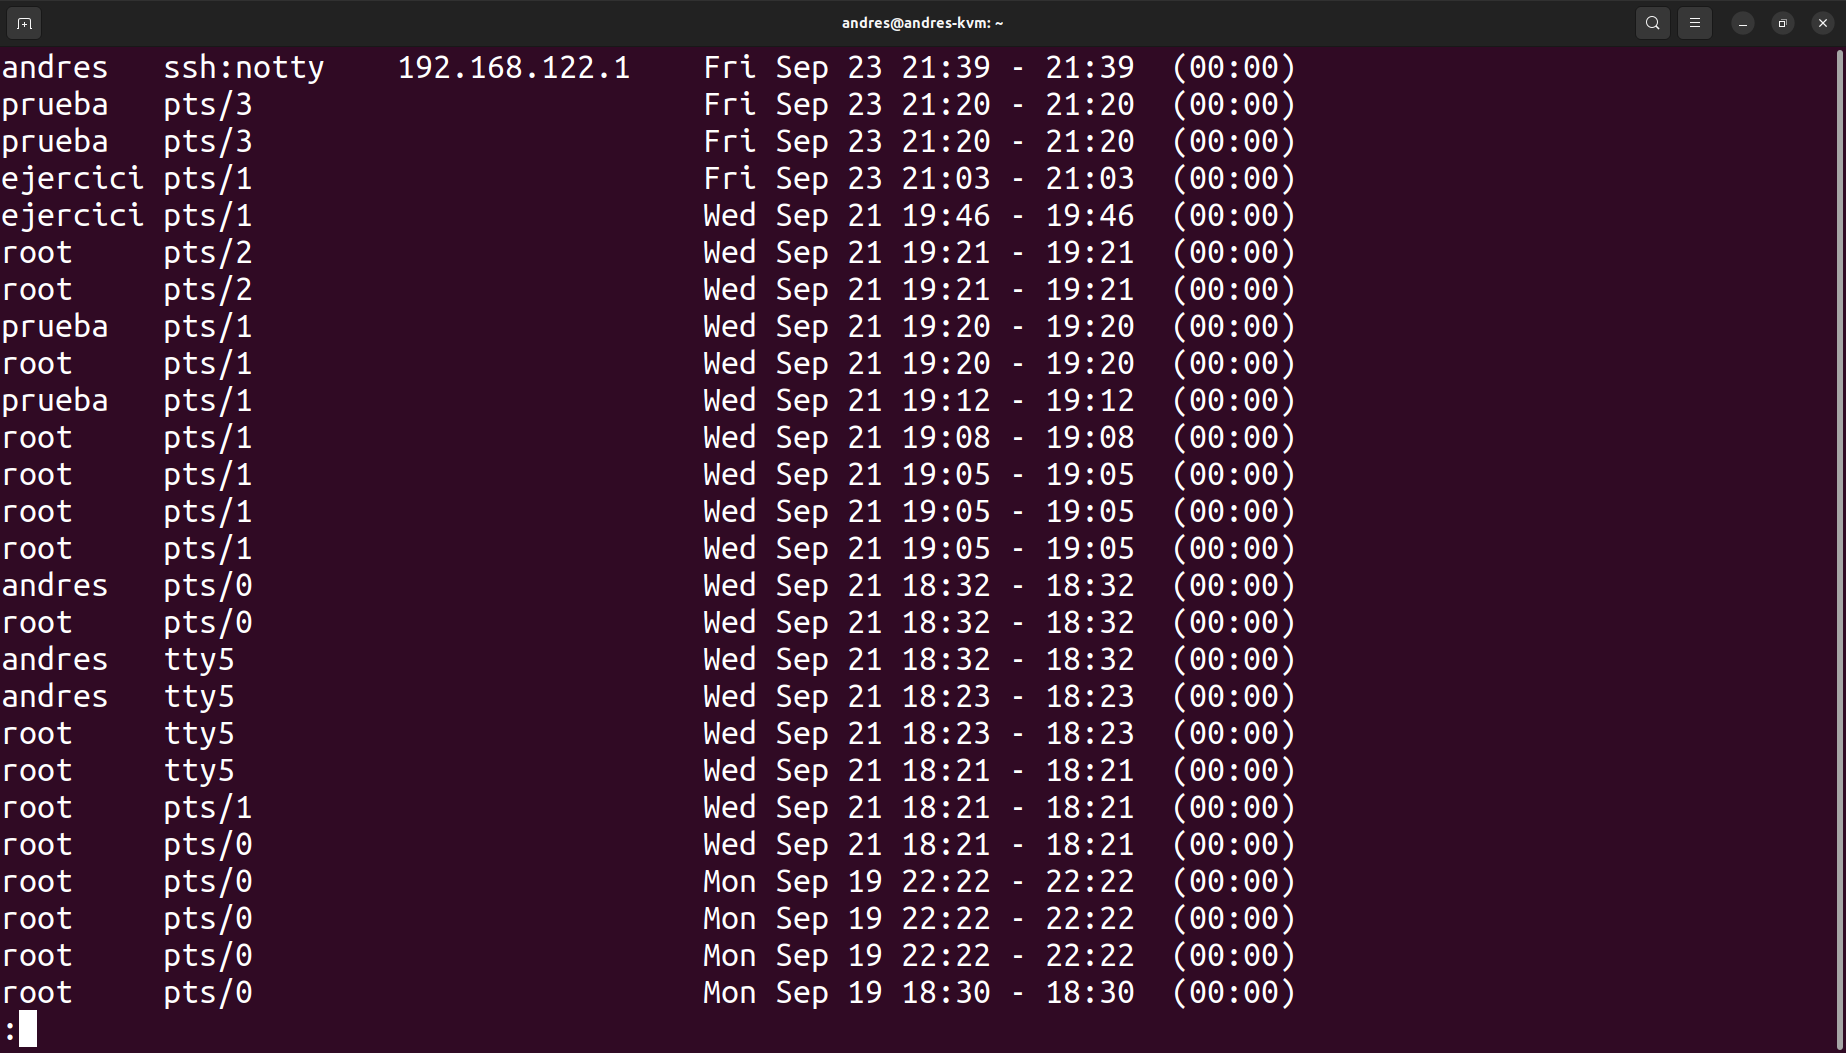
\includegraphics[width=\textwidth]{imagenes/lastbip.png}
\end{figure}

Como se puede ver, la dirección IP ``192.168.122.1'' ha intentado conectarse a la máquina con el usuario ``andres'' por SSH. 

\begin{figure}[H]
    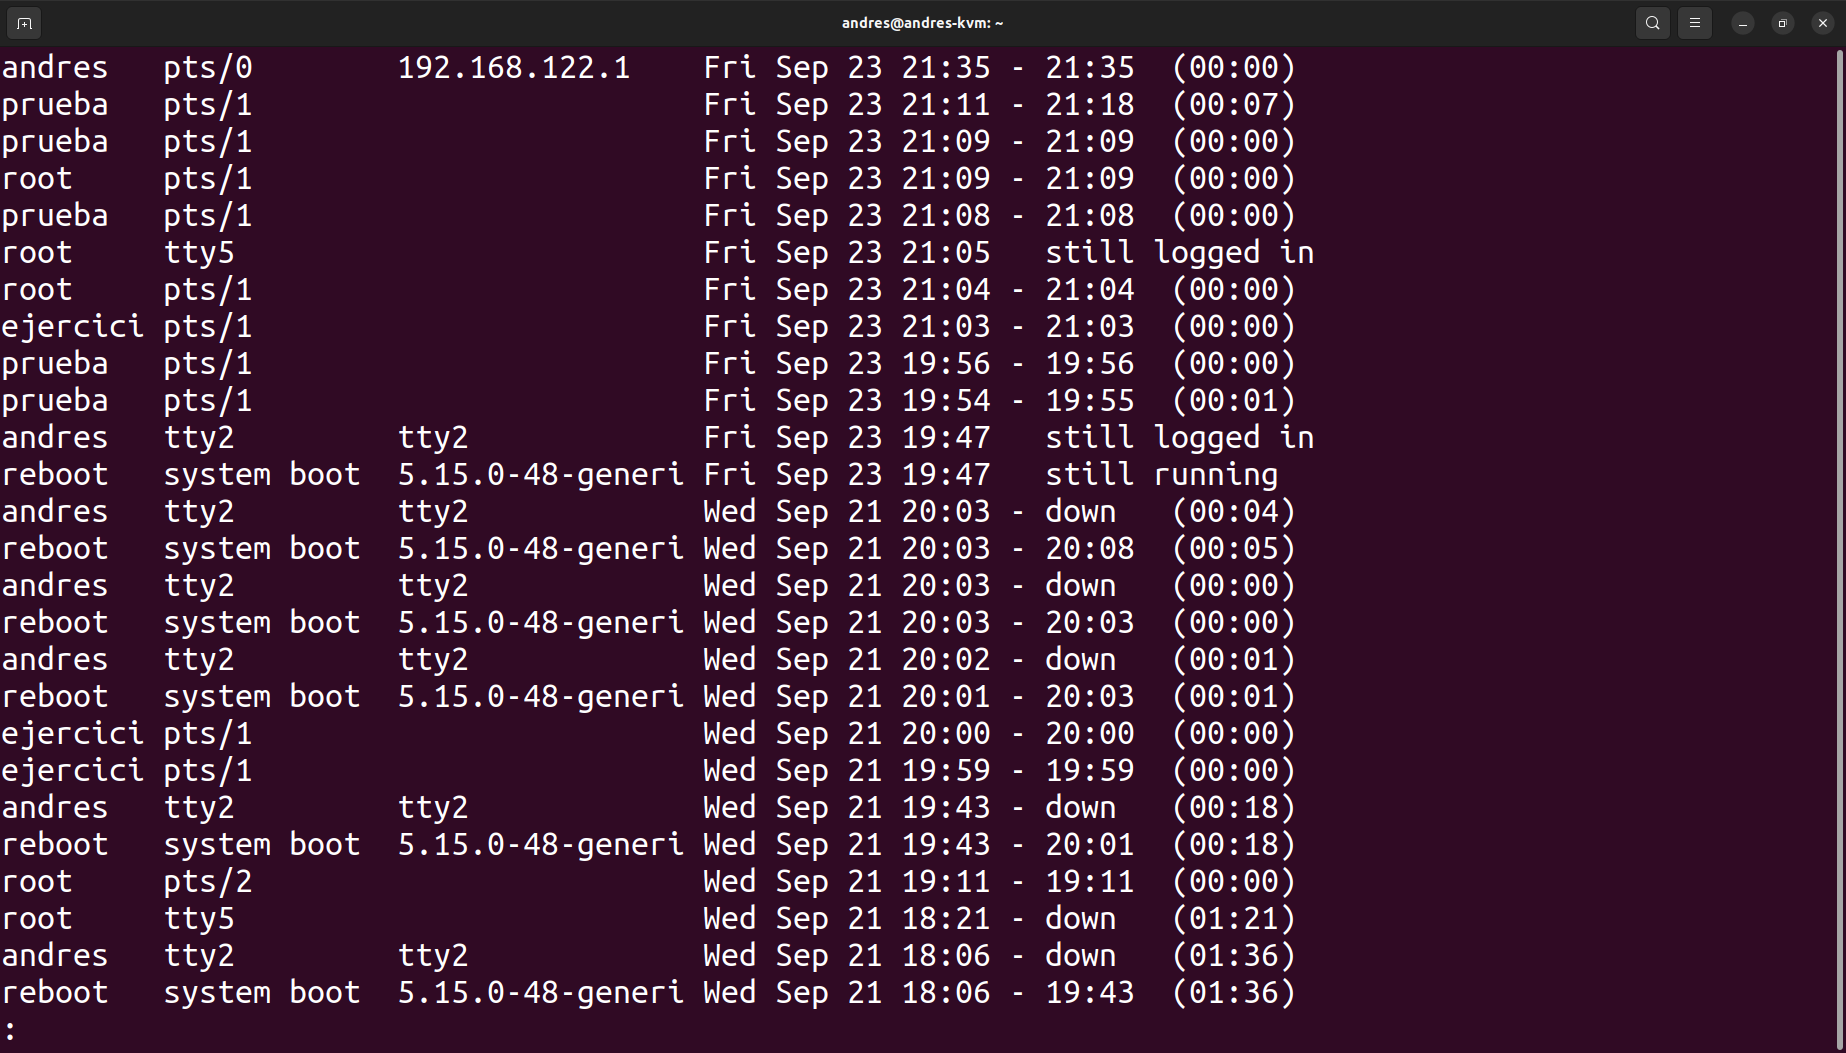
\includegraphics[width=\textwidth]{imagenes/lastip.png}
\end{figure}

Se puede observar que alguien ha entrado al sistema con SSH usando el usuario ``andres''.

\begin{figure}[H]
    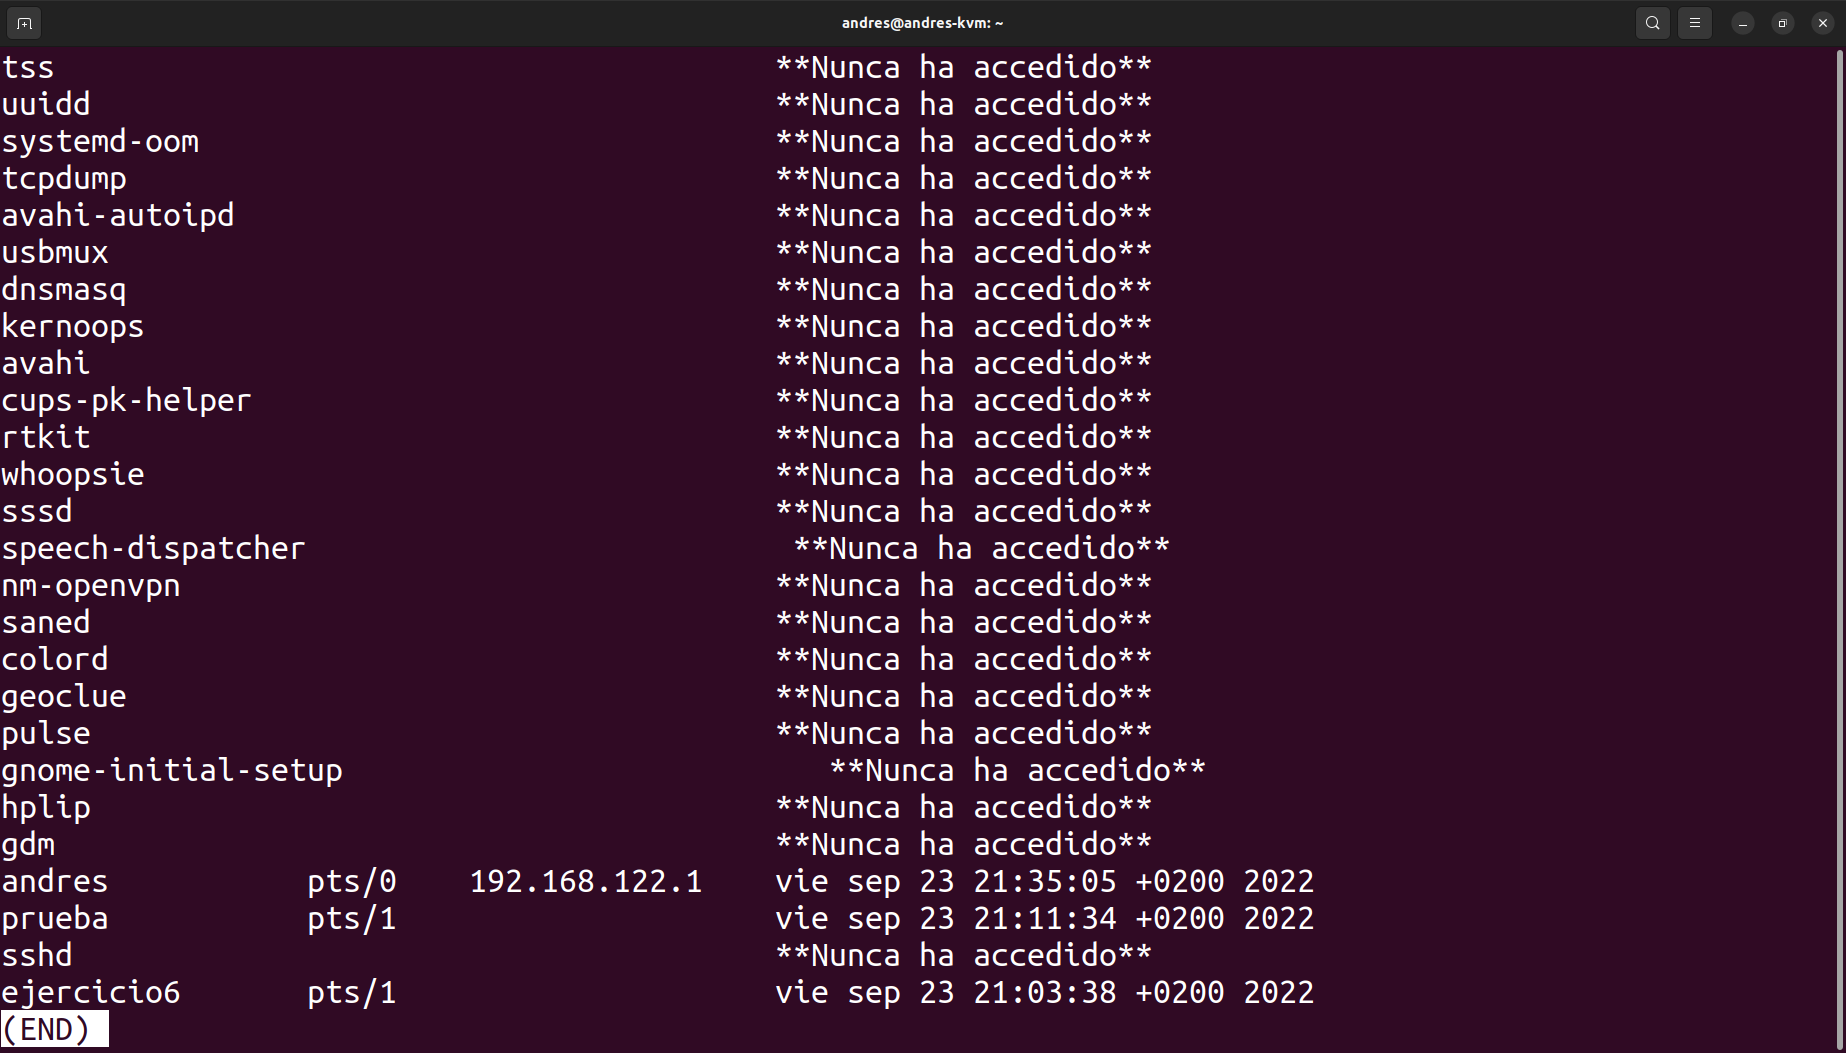
\includegraphics[width=\textwidth]{imagenes/lastlogip.png}
\end{figure}

Aquí también se puede observar que alguien ha accedido con la misma dirección IP anterior mediante SSH y ha conseguido iniciar sesión en el sistema.

Según estos datos, suponiendo que no hubiera sido yo, se podría decir que alguien ha intentado acceder al sistema y ha conseguido iniciar sesión como el usuario ``andres''. Una vez sacada esta conclusión, lo recomendable es detectar los cambios que ha realizado en el sistema y el tráfico de red para ver que posibles datos se ha podido llevar.
\end{document}
